\documentclass[%
    % draft,%
    xcolor=usenames,dvipsnames,svgnames%
]{beamer}

% \setbeameroption{show notes}
% \setbeameroption{show only notes}

\usetheme{eric}

\usepackage{xparse}

\usepackage[%
    backend    = biber,%
    style      = chem-acs,%
    autocite   = superscript,%
    backref    = true,%
    biblabel   = brackets,%
    doi        = true,%
    minnames   = 1,%
    maxnames   = 10,%
]{biblatex}
\addbibresource{../library.bib}
\addbibresource{../library2.bib}
\addbibresource{../paper_04/paper.bib}
\addbibresource{../paper_05/psi4numpy.bib}
\addbibresource{../paper_05/tutorial.bib}
\addbibresource{../5746059.bib}
\addbibresource{../5773968.bib}
\addbibresource{../in_preparation.bib}
\addbibresource{./presentation.bib}

\AtEveryCitekey{\iffootnote{\color{PittBlue}\tiny}{}}
\NewDocumentCommand{\nmfootfullcite}{m}{%
    \AtNextCite{%
        \let\thefootnote\relax
        \let\mkbibfootnote\mkbibfootnotetext
    }{%
        \footfullcite{#1}
    }
}

\usepackage{booktabs}
\usepackage{braket}
\usepackage{caption}
% \usepackage{showframe}
% \renewcommand\ShowFrameLinethickness{0.15pt}
% \renewcommand*\ShowFrameColor{\color{red}}
\usepackage{graphicx}
\usepackage{microtype}
\usepackage{minted}
\setminted{%
  autogobble=false,%
  breaklines=true,%
  fontsize=\footnotesize,%
  frame=none,%
  linenos=true,%
  mathescape=true,%
  python3=true,%
  texcomments=false,%
}
\usepackage[version=4]{mhchem}
\newcommand{\arlidimer}{\ce{Ar\bond{....}Li+}}
\usepackage[%
    separate-uncertainty = true,%
    multi-part-units = single,%
    range-units = single,%
    retain-explicit-plus = true,%
]{siunitx}
\usepackage{subcaption}
\usepackage{tabulary}
\usepackage{textcomp}

\NewDocumentCommand{\vect}{m}{%
        \ensuremath{\boldsymbol{\mathbf{#1}}}%
}%

% https://tex.stackexchange.com/a/98893/94717
\newenvironment{nscenter}
 {\parskip=0pt\par\nopagebreak\centering}
 {\par\noindent\ignorespacesafterend}

% https://tex.stackexchange.com/q/252586/94717
\newwrite\tempfile
\immediate\openout\tempfile=slidelist.txt
\newcounter{SlideNumber}
\addtobeamertemplate{frametitle}{}{%
  \stepcounter{SlideNumber}
  \immediate\write\tempfile{\theSlideNumber [\insertframenumber] \insertframetitle}
}

% \newcommand\pfour{\textsc{Psi4}}
\newcommand\pfour{Psi4}
% \newcommand\pfn{\textsc{Psi4NumPy}}
\newcommand\pfn{Psi4NumPy}
\newcommand\libresponse{\texttt{libresponse}}

\title{Decomposition of Intermolecular Interactions in \textit{Ab Initio} Spectroscopy}
\author{Eric Berquist}
\institute{
\includegraphics[width=1in]{./figures/pitt_logo.pdf}}
\date{March 23rd, 2018}

\begin{document}

\frame{
  \titlepage
}

\frame{
  \frametitle{Outcomes of this work}
  \note[item]{Why do we generally care about decomposing spectra? A sentence or two (spoken) about the bigger picture could serve as motivation for the methods development.}
  Thesis: It is possible to identify the contribution of specific molecular interactions to spectroscopic response.
  \tableofcontents
}

\note{\tiny\listofframes}

\begin{frame}
  \frametitle{Molecular spectroscopy is a probe of changes in a molecule's electronic and geometric state using electromagnetic radiation}
  \begin{nscenter}
    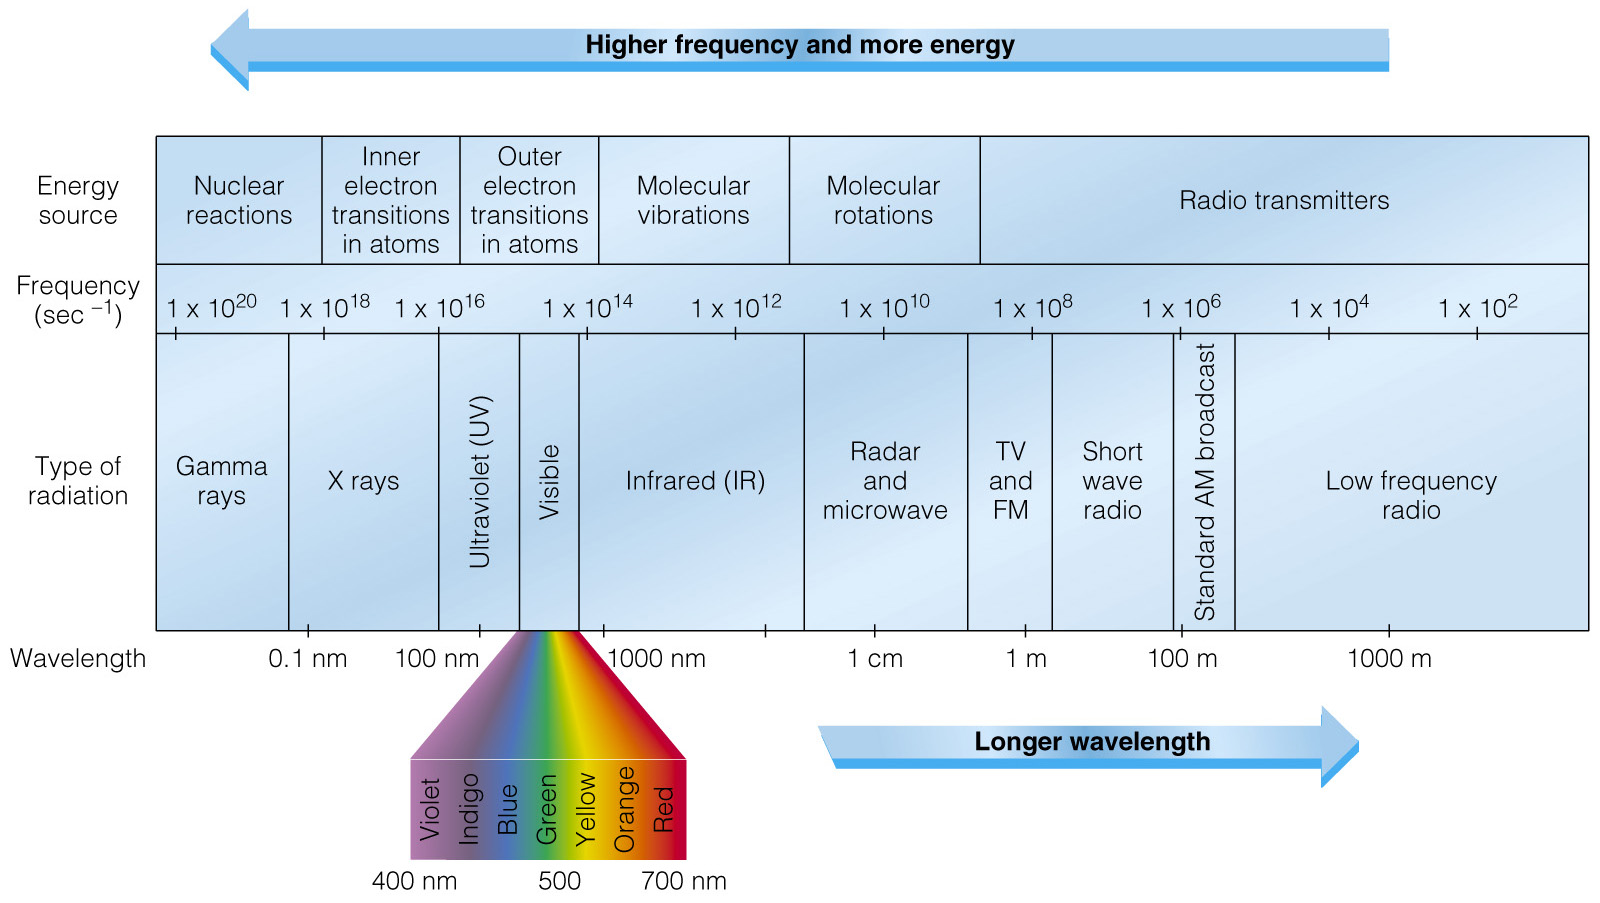
\includegraphics[width=\linewidth,keepaspectratio]{./figures/electromagnetic-spectrum.jpg}
  \end{nscenter}
  {\tiny\url{http://hrsbstaff.ednet.ns.ca/benoitn/chem11/units/1.\%20Atomic\%20Theory/e_config/spectra/electromagnetic-spectrum.jpg}}
  \note[item]{Tom comment: "not excited states, just looking at polarizability" -- this statement did not make sense to me}
  \note[item]{Response: wavelengths associated with frequency-dependent polarizability are also associated with UV/vis; probably don't need to mention this}
\end{frame}

\section{Decomposition of harmonic vibrational frequencies into physically-intuitive terms}

\begin{frame}[fragile]
  \frametitle{\protect{Infrared spectroscopy is sensitive to the presence of \ce{CO2} in ionic liquids}}
  \note[item]{For example, ...}
  \note[item]{\ce{CO2} asymmetric stretch lies in an isolated spectral window}
  \begin{nscenter}
    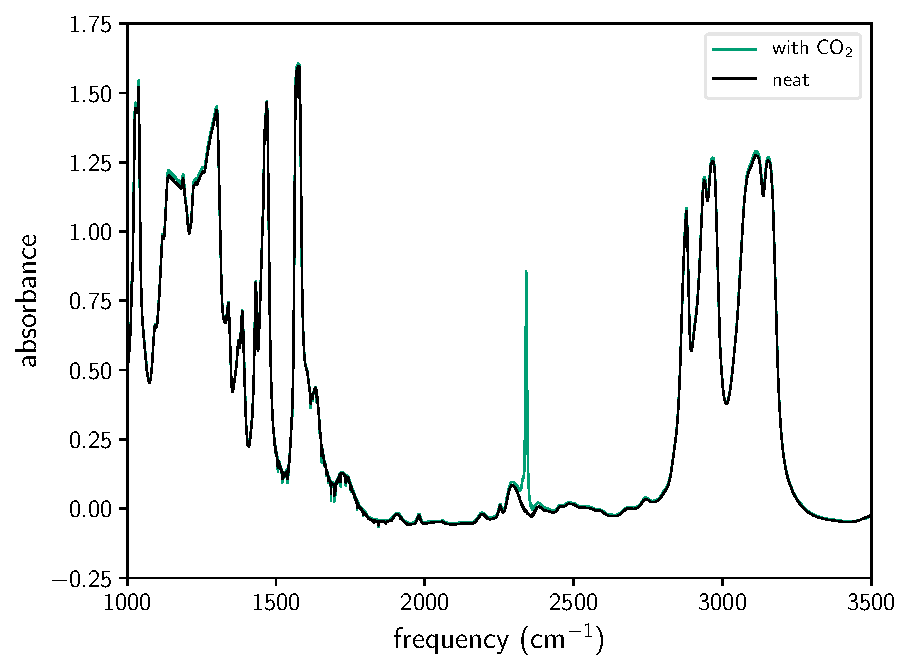
\includegraphics[width=\linewidth,keepaspectratio]{./figures/experimental_spectra_TfO.pdf}
  \end{nscenter}
\end{frame}

\begin{frame}[fragile]
  \frametitle{\protect{Understanding \ce{CO2} solvation by ionic liquids is important for carbon capture}}
  \note[item]{Why these? Water tolerant, fairly good CO2 capture already, experimentally studied/validated}
  \note[item]{desirable properties of ionic liquids: solvation energy, reversible absorption}
  \note[item]{point out nomenclature}
  \note[item]{room temperature}
  \note[item]{experimentally interesting to change the anion because of correlation with \emph{solubility}}
  Example ionic liquids (ILs) studied experimentally:
  \begin{table}
    \centering
    \begin{tabulary}{1.00\linewidth}{CCCC}
      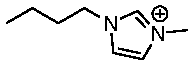
\includegraphics[scale=1.00]{./figures/lewis_C4C1im.pdf} & 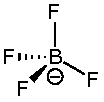
\includegraphics[scale=1.00]{./figures/lewis_BF4.pdf} & 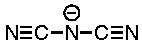
\includegraphics[scale=1.00]{./figures/lewis_DCA.pdf} & 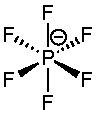
\includegraphics[scale=1.00]{./figures/lewis_PF6.pdf} \\
      \ce{[C4C1im]+} & \ce{[BF4]-} & \ce{[DCA]-} & \ce{[PF6]-} \\
      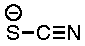
\includegraphics[scale=1.00]{./figures/lewis_SCN.pdf} & 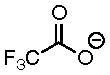
\includegraphics[scale=1.00]{./figures/lewis_TFA.pdf} & 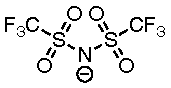
\includegraphics[scale=1.00]{./figures/lewis_Tf2N.pdf} & 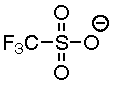
\includegraphics[scale=1.00]{./figures/lewis_TfO.pdf} \\
      \ce{[SCN]-} & \ce{[TFA]-} & \ce{[Tf2N]-} & \ce{[TfO]-}
    \end{tabulary}
  \end{table}
  \nmfootfullcite{Brinzer2015}
\end{frame}

% method 1
  % \begin{figure}
  %   \centering
  %   \begin{subfigure}[b]{0.25\linewidth}
  %     \centering
  %     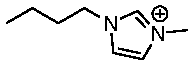
\includegraphics[scale=1.00]{./figures/lewis_C4C1im.pdf}
  %     \caption*{\ce{[C4C1im]+}}
  %   \end{subfigure}
  %   % \begin{subfigure}[b]{0.25\linewidth}
  %   %   \centering
  %   %   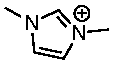
\includegraphics[scale=1.00]{./figures/lewis_C1C1im.pdf}
  %   %   \caption*{\ce{[C1C1im]+}}
  %   % \end{subfigure}
  %   \begin{subfigure}[b]{0.25\linewidth}
  %     \centering
  %     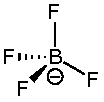
\includegraphics[scale=1.00]{./figures/lewis_BF4.pdf}
  %     \caption*{\ce{[BF4]-}}
  %   \end{subfigure}
  %   \begin{subfigure}[b]{0.25\linewidth}
  %     \centering
  %     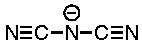
\includegraphics[scale=1.00]{./figures/lewis_DCA.pdf}
  %     \caption*{\ce{[DCA]-}}
  %   \end{subfigure}
  %   \begin{subfigure}[b]{0.25\linewidth}
  %     \centering
  %     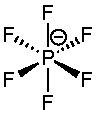
\includegraphics[scale=1.00]{./figures/lewis_PF6.pdf}
  %     \caption*{\ce{[PF6]-}}
  %   \end{subfigure}
  %   \begin{subfigure}[b]{0.25\linewidth}
  %     \centering
  %     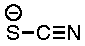
\includegraphics[scale=1.00]{./figures/lewis_SCN.pdf}
  %     \caption*{\ce{[SCN]-}}
  %   \end{subfigure}
  %   \begin{subfigure}[b]{0.25\linewidth}
  %     \centering
  %     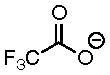
\includegraphics[scale=1.00]{./figures/lewis_TFA.pdf}
  %     \caption*{\ce{[TFA]-}}
  %   \end{subfigure}
  %   \begin{subfigure}[b]{0.25\linewidth}
  %     \centering
  %     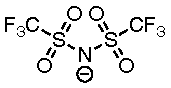
\includegraphics[scale=1.00]{./figures/lewis_Tf2N.pdf}
  %     \caption*{\ce{[Tf2N]-}}
  %   \end{subfigure}
  %   \begin{subfigure}[b]{0.25\linewidth}
  %     \centering
  %     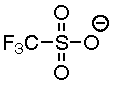
\includegraphics[scale=1.00]{./figures/lewis_TfO.pdf}
  %     \caption*{\ce{[TfO]-}}
  %   \end{subfigure}
  % \end{figure}
% method 2
  % \begin{columns}
  %   \column{0.25\linewidth}
  %   \begin{minipage}[c]{1.0\linewidth}
  %     \centering
  %     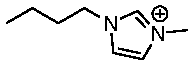
\includegraphics[scale=1.00]{./figures/lewis_C4C1im.pdf}
  %     \ce{[C4C1im]+}
  %     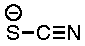
\includegraphics[scale=1.00]{./figures/lewis_SCN.pdf}
  %     \ce{[SCN]-}
  %   \end{minipage}
  %   \column{0.25\linewidth}
  %   \begin{minipage}[c]{1.0\linewidth}
  %     \centering
  %     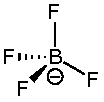
\includegraphics[scale=1.00]{./figures/lewis_BF4.pdf}
  %     \ce{[BF4]-}
  %     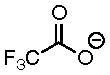
\includegraphics[scale=1.00]{./figures/lewis_TFA.pdf}
  %     \ce{[TFA]-}
  %   \end{minipage}
  %   \column{0.25\linewidth}
  %   \begin{minipage}[c]{1.0\linewidth}
  %     \centering
  %     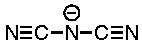
\includegraphics[scale=1.00]{./figures/lewis_DCA.pdf}
  %     \ce{[DCA]-}
  %     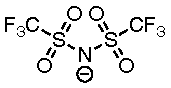
\includegraphics[scale=1.00]{./figures/lewis_Tf2N.pdf}
  %     \ce{[Tf2N]-}
  %   \end{minipage}
  %   \column{0.25\linewidth}
  %   \begin{minipage}[c]{1.0\linewidth}
  %     \centering
  %     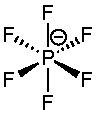
\includegraphics[scale=1.00]{./figures/lewis_PF6.pdf}
  %     \ce{[PF6]-}
  %     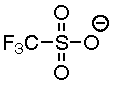
\includegraphics[scale=1.00]{./figures/lewis_TfO.pdf}
  %     \ce{[TfO]-}
  %   \end{minipage}
  % \end{columns}
% method 3
  % \begin{table}
  %   \centering
  %   \begin{tabulary}{1.00\linewidth}{CCCC}
  %     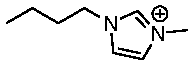
\includegraphics[scale=1.00]{./figures/lewis_C4C1im.pdf} & 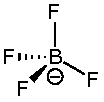
\includegraphics[scale=1.00]{./figures/lewis_BF4.pdf} & 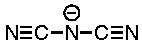
\includegraphics[scale=1.00]{./figures/lewis_DCA.pdf} & 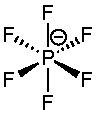
\includegraphics[scale=1.00]{./figures/lewis_PF6.pdf} \\
  %     \ce{[C4C1im]+} & \ce{[BF4]-} & \ce{[DCA]-} & \ce{[PF6]-} \\
  %     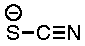
\includegraphics[scale=1.00]{./figures/lewis_SCN.pdf} & 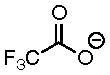
\includegraphics[scale=1.00]{./figures/lewis_TFA.pdf} & 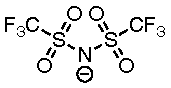
\includegraphics[scale=1.00]{./figures/lewis_Tf2N.pdf} & 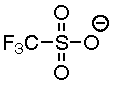
\includegraphics[scale=1.00]{./figures/lewis_TfO.pdf} \\
  %     \ce{[SCN]-} & \ce{[TFA]-} & \ce{[Tf2N]-} & \ce{[TfO]-}
  %   \end{tabulary}
  % \end{table}
\begin{frame}
  \frametitle{Solvatochromic shift originates from varying the ionic liquid anion}
  \begin{nscenter}
    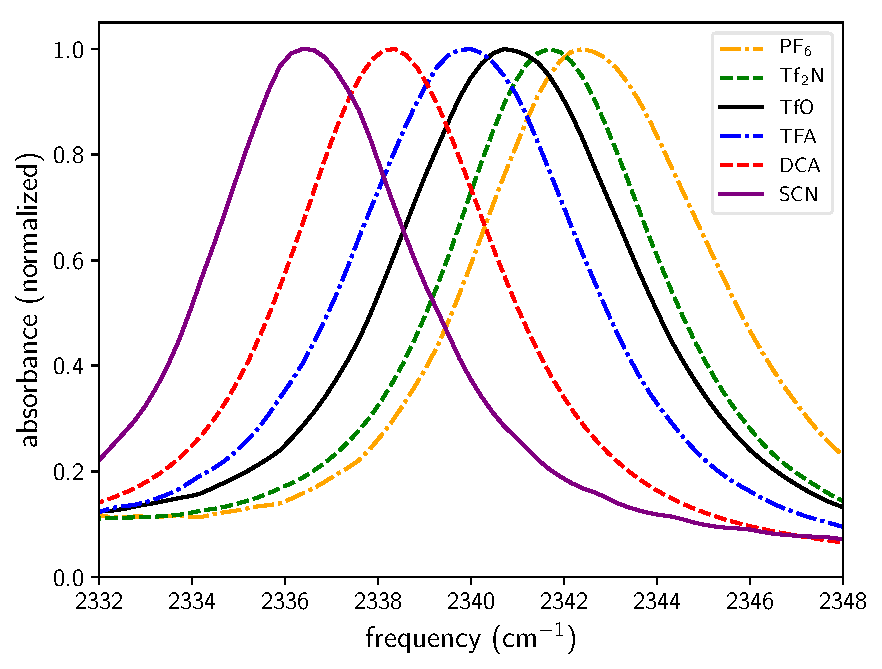
\includegraphics[scale=0.65]{./figures/experimental_spectra_shifting.pdf}
  \end{nscenter}
  \scriptsize
  experiment, \ce{[C4C1im]+}
\end{frame}

\begin{frame}
  \frametitle{Model calculations qualitatively reproduce trends in the solvatochromic shift}
  \note[item]{Experimental cation is C4C1im, computational cation is C1C1im}
  \note[item]{quantum chemistry connects frequencies to structure}
  % 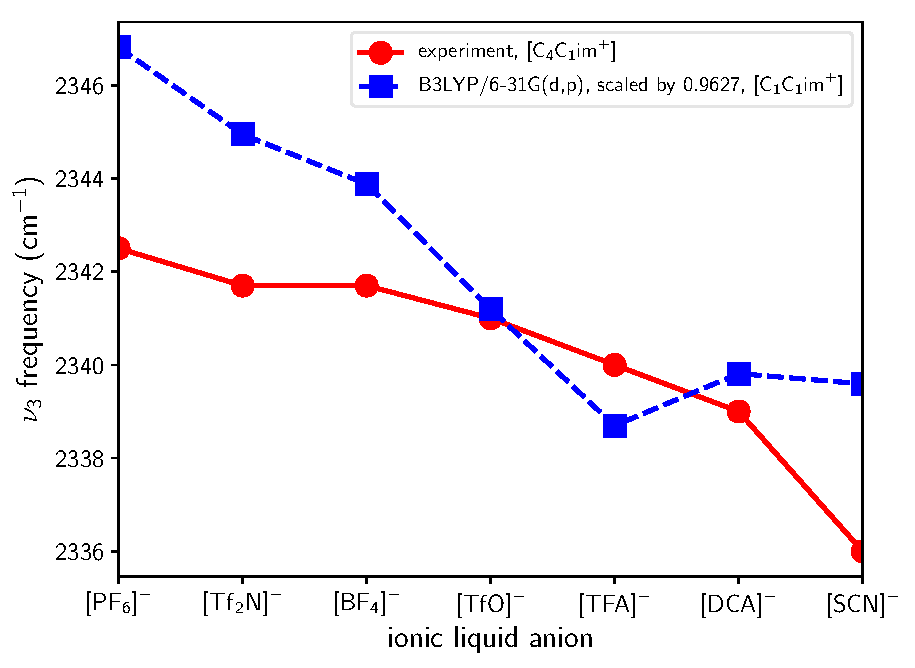
\includegraphics[width=\linewidth,keepaspectratio]{./figures/frequencies_calc_vs_expt1.pdf}
  \begin{nscenter}
    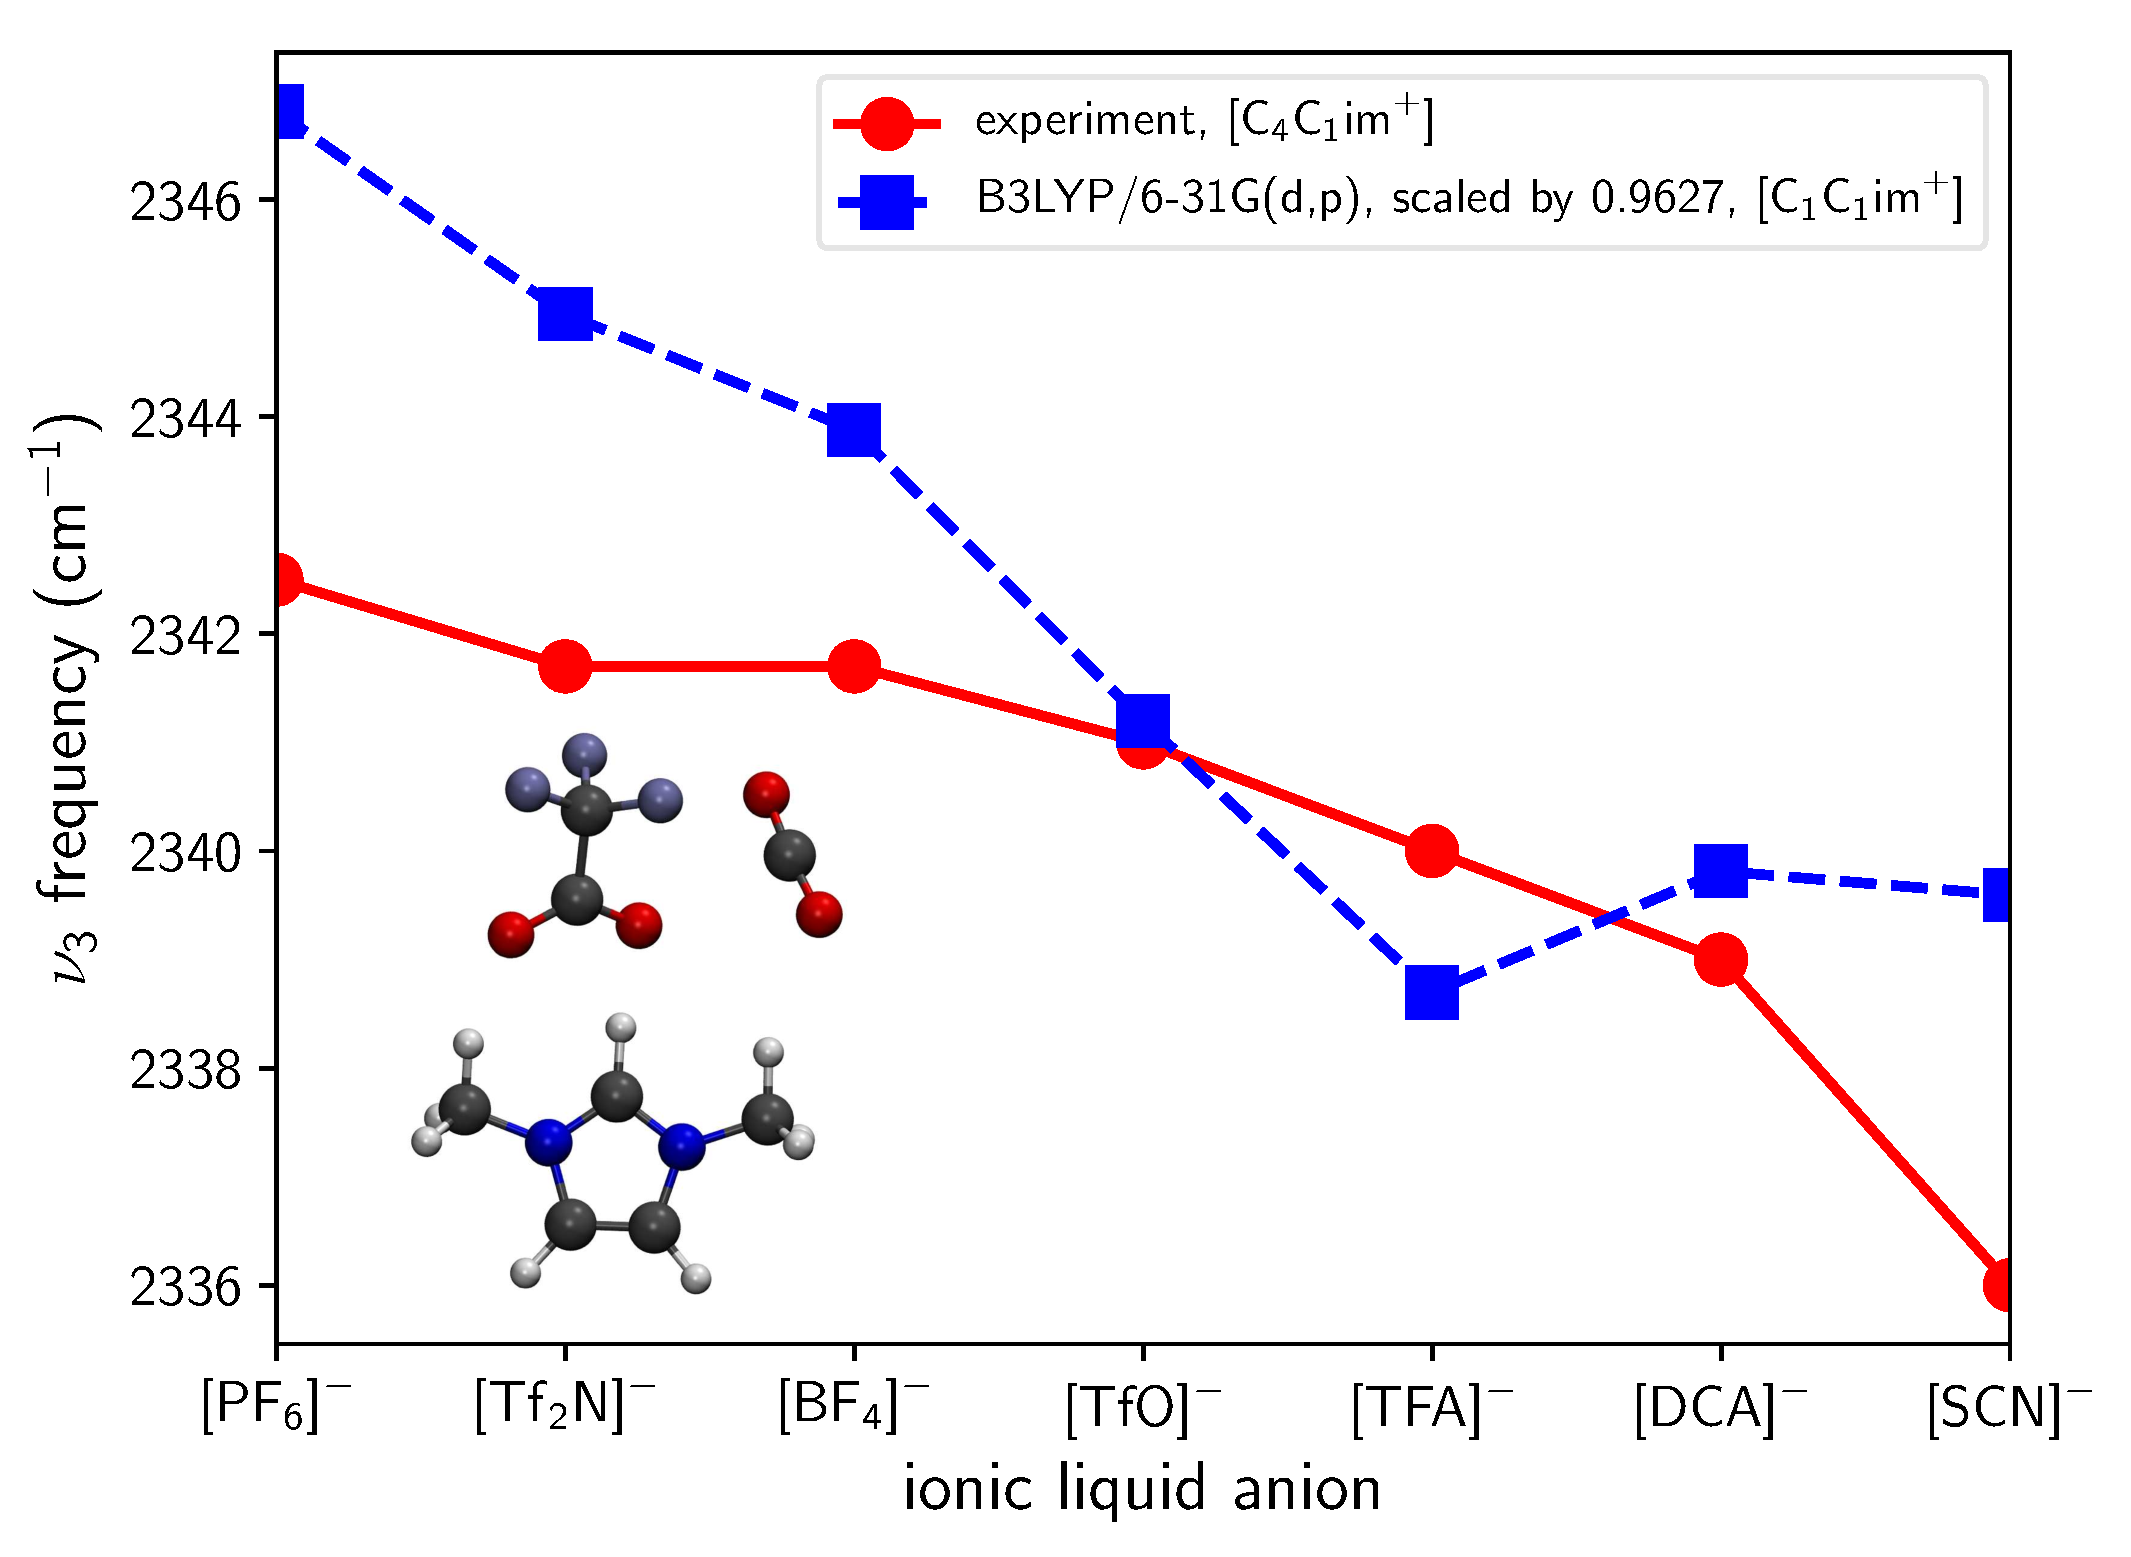
\includegraphics[width=\linewidth,keepaspectratio]{./figures/frequencies_calc_vs_expt1_combined2.pdf}
  \end{nscenter}
  % \nmfootfullcite{Brinzer2015}
\end{frame}

\begin{frame}
  % \frametitle{ALMO-EDA enables understanding the physical basis for the solvatochromic shift}
  % \frametitle{What is the physical basis for the solvatochromic shift?}
  % \frametitle{Energy decomposition analysis provides an intuitive assignment of intermolecular interactions to physical terms}
  \frametitle{Energy decomposition analysis can explain the physical basis for the solvatochromic shift}
  \note[item]{Performed using absolutely localized molecular orbitals (ALMO-EDA), a ``bottom-up'' localization technique that prevents charge transfer by construction}
  \note[item]{How an ALMO is constructed}
  \note[item]{Intermediate wavefunction!}
  \note[item]{Can move on the ALMO potential energy surface}
  \note[item]{Explanation of Pauli repulsion, signs of terms}
  For two arbitrary fragments A and B (such as a \ce{CO2} molecule and a combined IL cation and anion), construct \alert{absolutely localized molecular orbitals} (ALMOs) on each fragment, then perform projected SCF for molecular interactions, SCF(MI):
  \begin{table}
    \centering
    \begin{tabular}{ccc}
      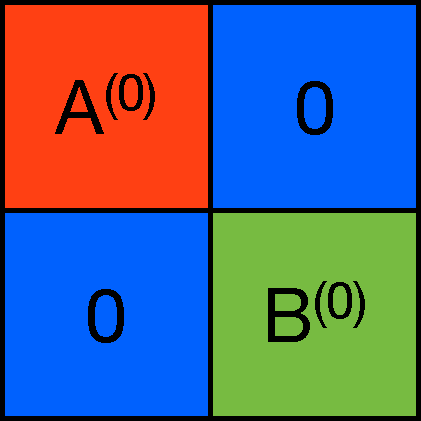
\includegraphics[scale=0.30]{./figures/block_1.pdf} & 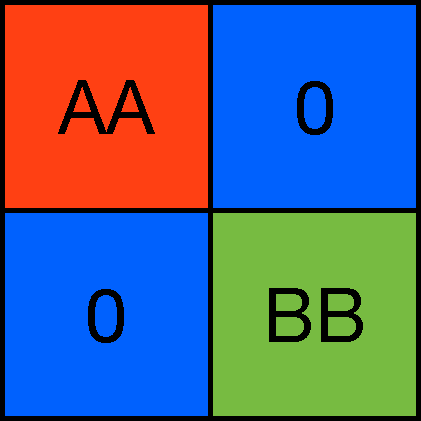
\includegraphics[scale=0.30]{./figures/block_2.pdf} & 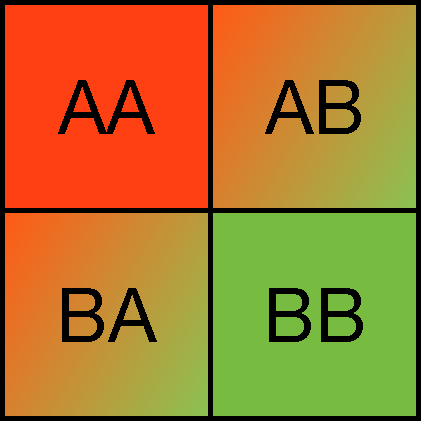
\includegraphics[scale=0.30]{./figures/block_3.pdf} \\
      frozen interaction (frz) & polarization (pol) & charge transfer (CT) \\
      \((\vect{1} - \vect{\sigma})^{\dagger} \vect{H}^{(0)} (\vect{1} - \vect{\sigma})\) & \((\vect{1} - \vect{\sigma})^{\dagger} \vect{H} (\vect{1} - \vect{\sigma})\) & \(\vect{H}\)
    \end{tabular}
  \end{table}
  \uncover<2->{Translate}
  \begin{equation*}
    \Delta E_{\text{int}} = \Delta E_{\text{geom}} + \Delta E_{\text{frz}} + \Delta E_{\text{pol}} + \Delta E_{\text{CT}}
  \end{equation*}
  \uncover<2->{%
  into
  \begin{equation*}
    \omega_{\text{tot}} = \omega_{\text{free}} + \Delta \omega_{\text{geom}} + \Delta \omega_{\text{frz}} + \Delta \omega_{\text{pol}} + \Delta \omega_{\text{CT}}
  \end{equation*}
  }%
\end{frame}

\note{If going to talk about the geometry mechanism and the curvature mechanism, it should go here?}

\begin{frame}[fragile]
  \frametitle{\protect{The \ce{CO2} asymmetric stretch solvatochromic shift is caused by charge transfer-driven geometric distortion}}
  \note[item]{These frequencies are unscaled}
  \begin{nscenter}
    % 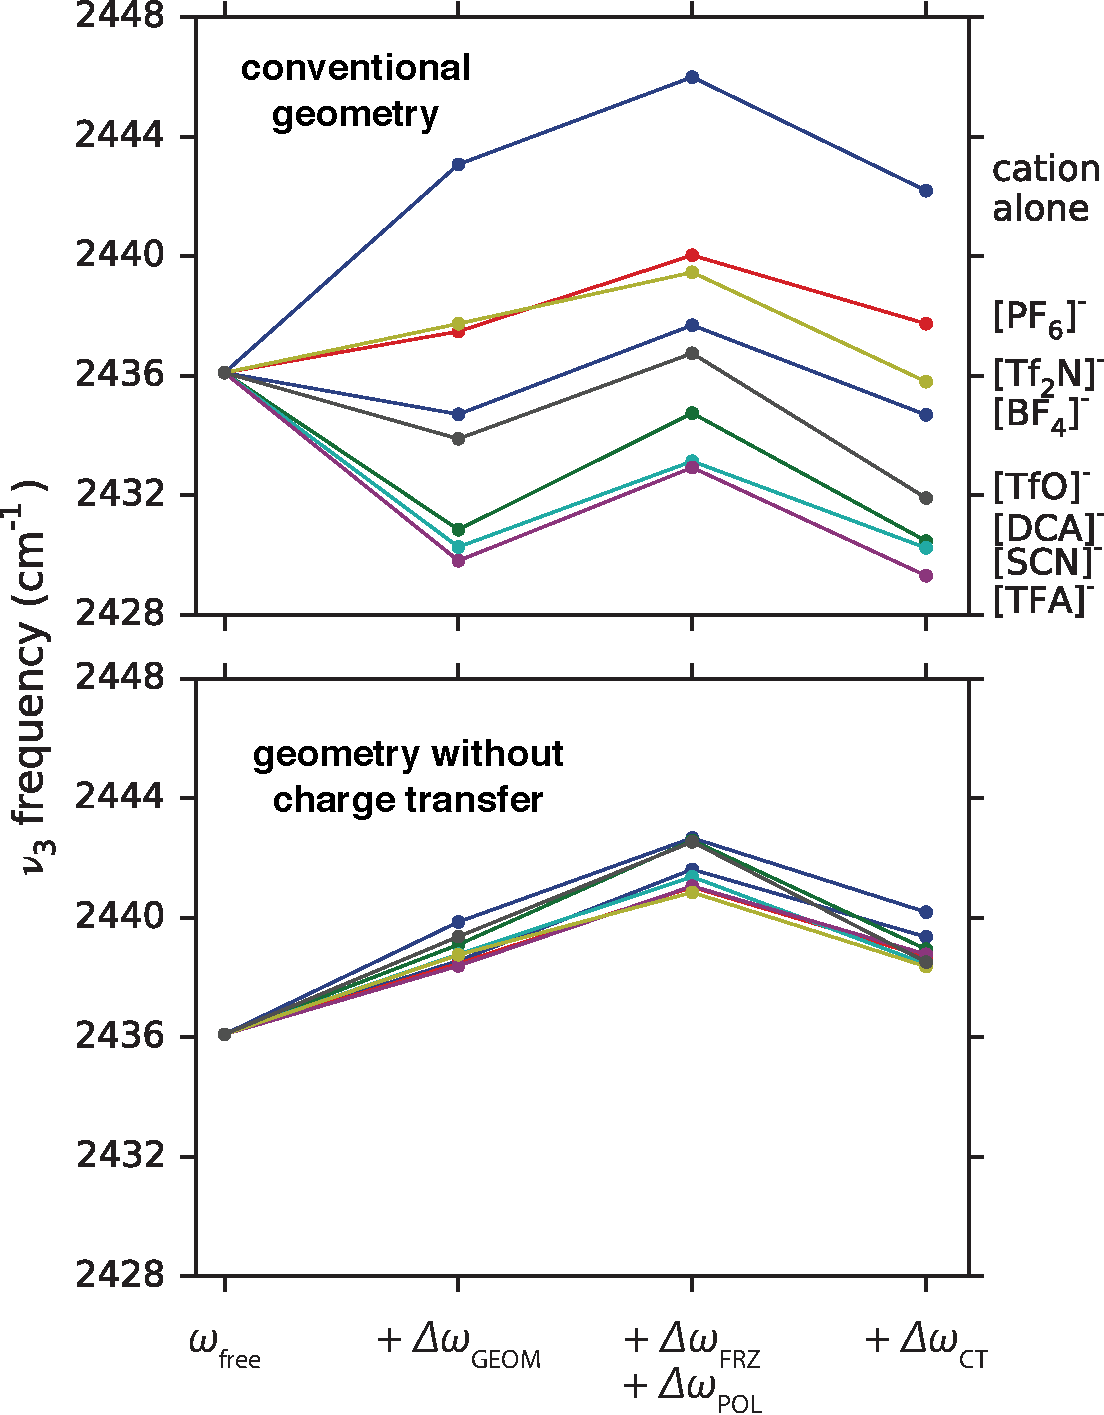
\includegraphics[scale=0.28]{./figures/ionic_liquid_geometry_dependence_on_ct.pdf}
    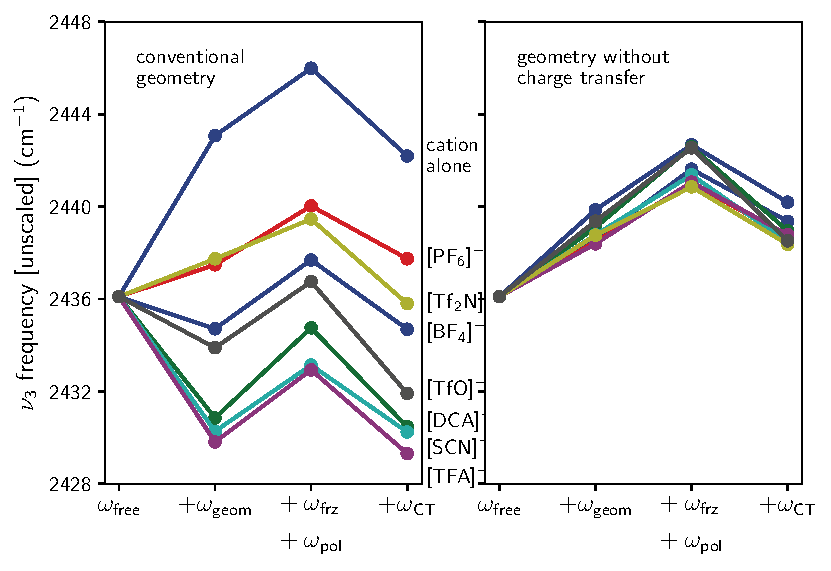
\includegraphics[scale=0.70]{./figures/00_all.pdf}
  \end{nscenter}
  {\scriptsize B3LYP/6-31G(d,p); cation is \ce{[C1C1im]+}}
\end{frame}

\begin{frame}
  \frametitle{Conclusion: spectra decomposition is an integral part of the experimental-computational workflow}
  \note[item]{cite Daly papers}
  \begin{columns}
    \column{0.60\textwidth}
    % 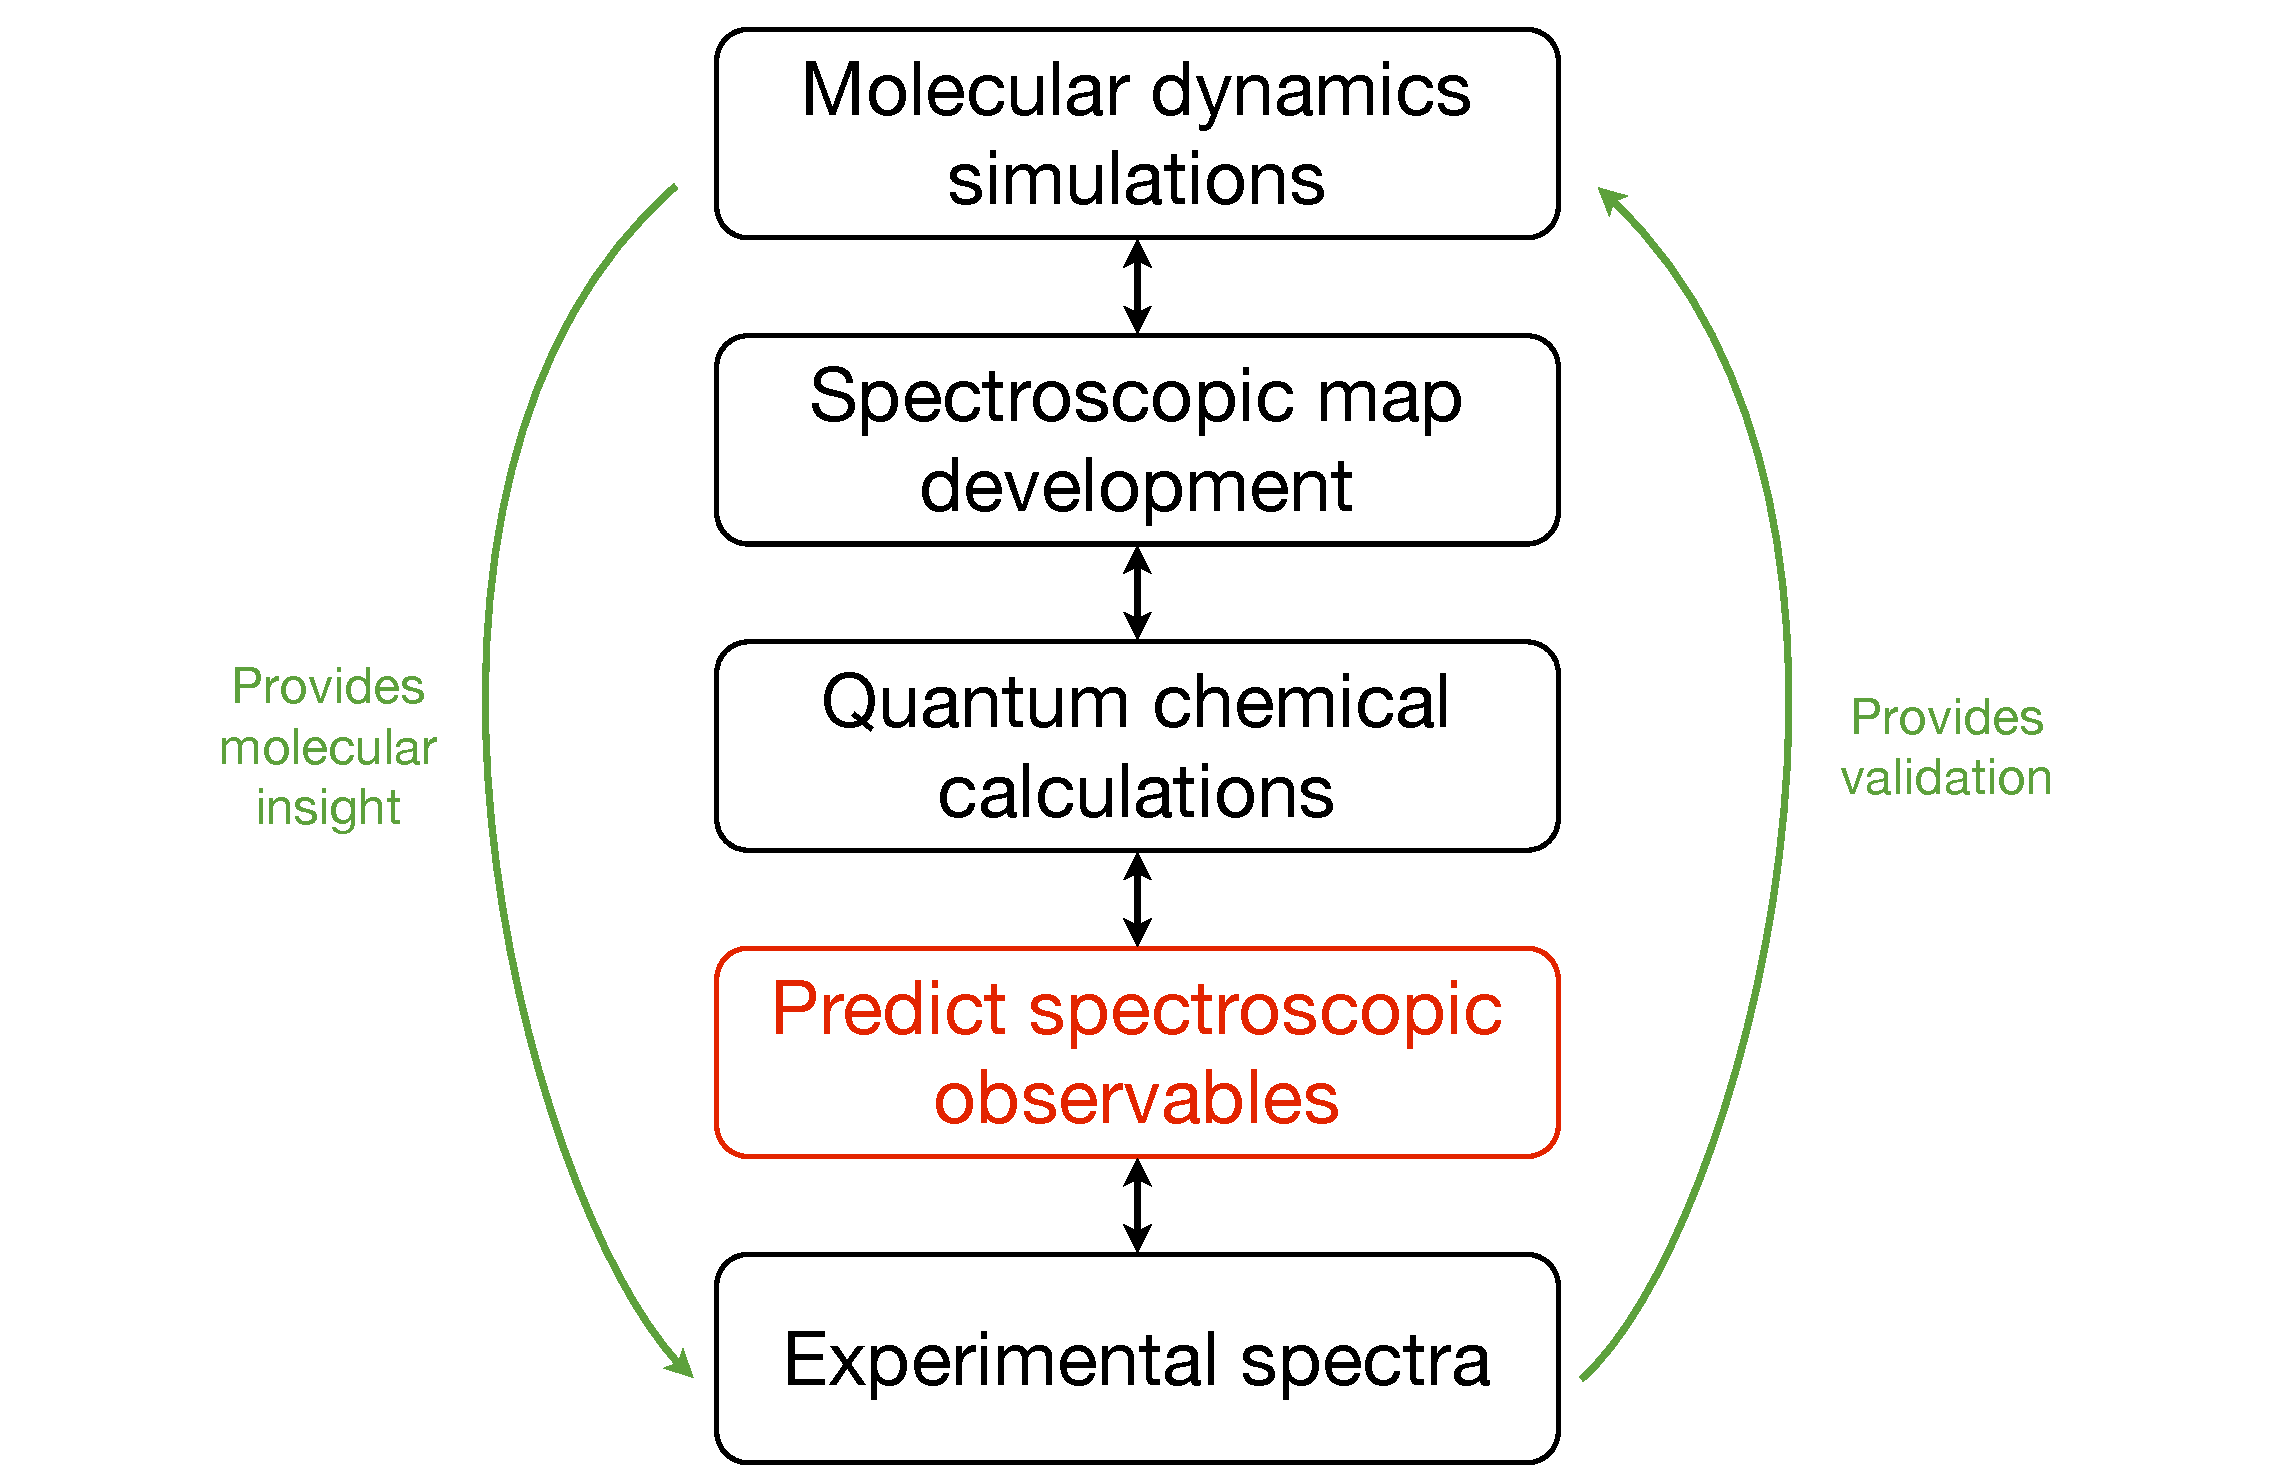
\includegraphics[scale=0.30]{./figures/workflow.pdf}
    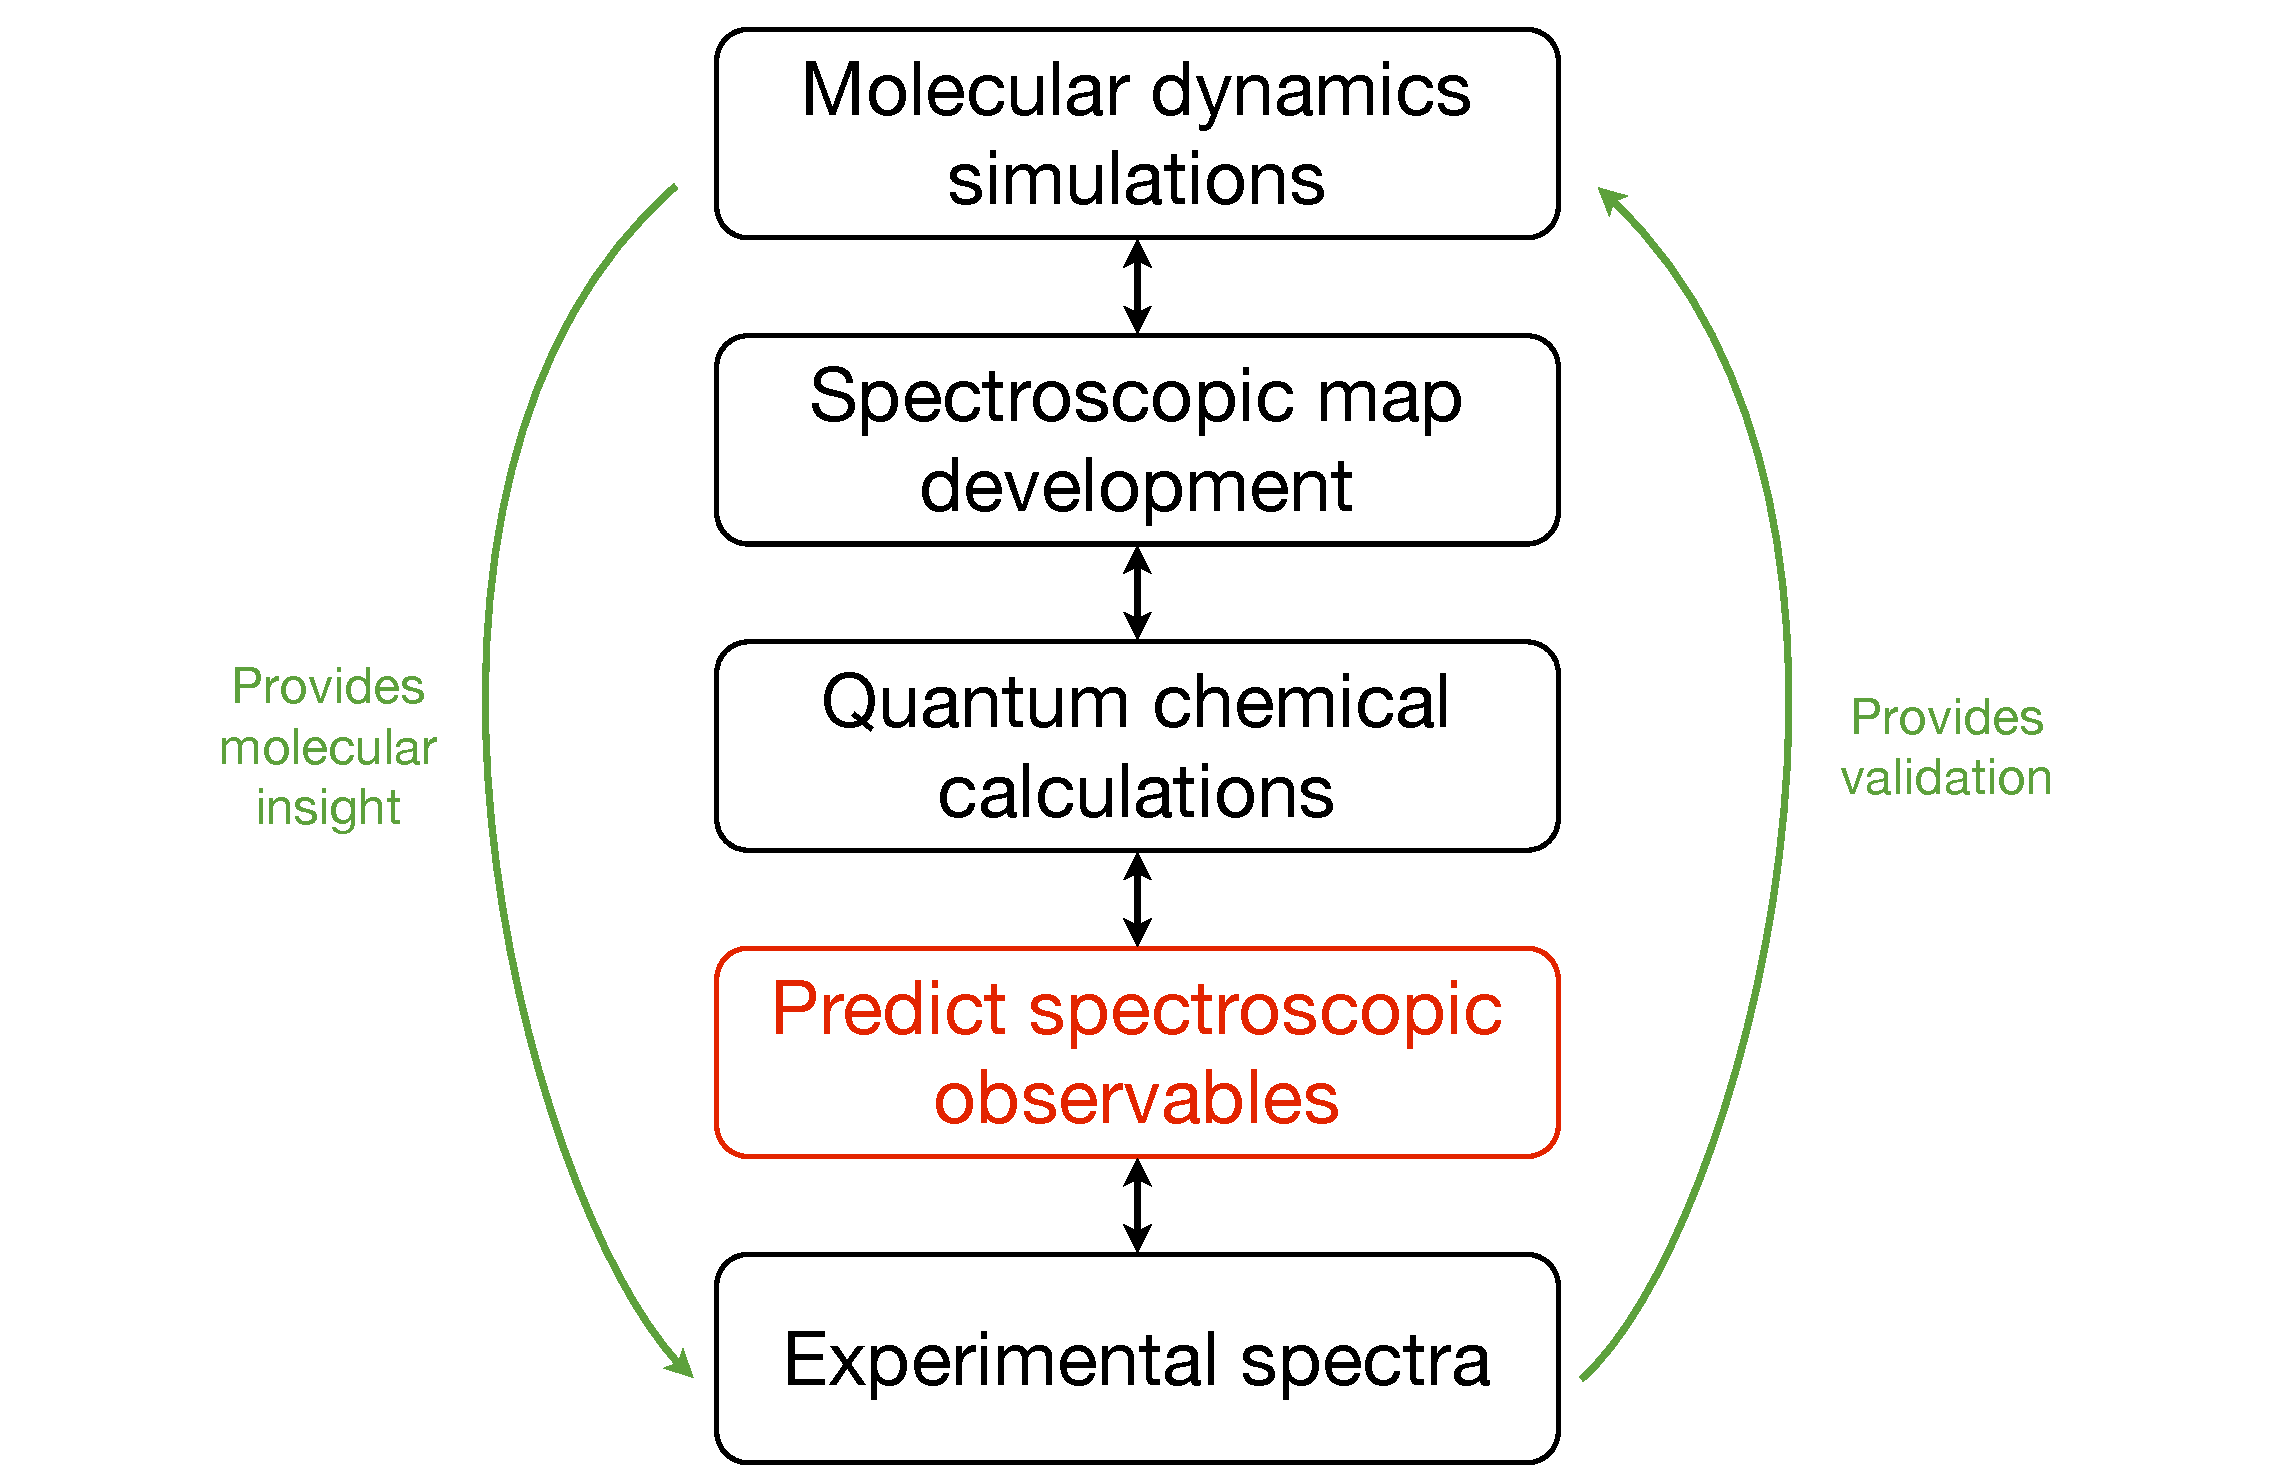
\includegraphics[width=\linewidth,keepaspectratio]{./figures/workflow.pdf}
    \column{0.40\textwidth}
    \begin{itemize}
    \item Construct empirical spectra-property relationships based on most significant interactions
    \item Test physical basis for experimental hypotheses (Stark effect, electrocatalysis)
    \end{itemize}
  \end{columns}
  \nmfootfullcite{Daly2016}
  \nmfootfullcite{Berquist2017}
\end{frame}

\begin{frame}
  \frametitle{Problem: the approach for decomposing vibrational frequencies is not generally applicable to other properties}
  \note[item]{What's the value of spectroscopy decomposition?}
  \note[item]{Want the ability to build structure-spectra relationships for any type of spectroscopy, leading to spectra-property relationships}
  Originally based on numerical differentiation using finite difference. Starting from a perturbation expansion
  \begin{equation*}
    \label{eq:maclaurin-expansion}
    \begin{aligned}
      E(P) &= \sum_{n = 0}^{\infty} \frac{1}{n!} \left. \frac{\partial^{n} E}{\partial P^{n}} \right|_{P = 0} \cdot P^{n} \\
      % &= \sum_{n = 0}^{\infty} \frac{1}{n!} E^{(n)} \cdot P^{n} \\
      &= E^{(0)} + E^{(1)} \cdot P + \frac{1}{2} E^{(2)} \cdot P^{2} + \frac{1}{6} E^{(3)} \cdot P^{3} + \dots,
    \end{aligned}
  \end{equation*}
  if the perturbation is an applied electric field \(\mathbf{F}\),
  \begin{equation*}
    \label{eq:electric-field-expansion}
    E(\mathbf{F}) = E_{0} + \mu_{i} \cdot F_{i} + \frac{1}{2} \alpha_{ij} \cdot F_{i}F_{j} + \frac{1}{6} \beta_{ijk} \cdot F_{i}F_{j}F_{k} + \frac{1}{24} \gamma_{ijkl} \cdot F_{i}F_{j}F_{k}F_{l} + \dots,
  \end{equation*}
  a component of the polarizability from 1st-order finite difference is
  \begin{equation*}
    \label{eq:finite-difference-polarizability}
    \alpha_{xz}(h_{x}) = \frac{\mu_{z}(\frac{1}{2}h_{x}) - \mu_{z}(\frac{1}{2}h_{x})}{h_{x}}.
  \end{equation*}
\end{frame}

\begin{frame}
  \frametitle{Numerical differentiation can give unphysical results}
  \note[item]{One example why the original approach is not generally applicable...}
  \note[item]{One problem with numerical differentiation is...}
  \note[item]{Mention other issues with numerical differentiation}
  \begin{nscenter}
    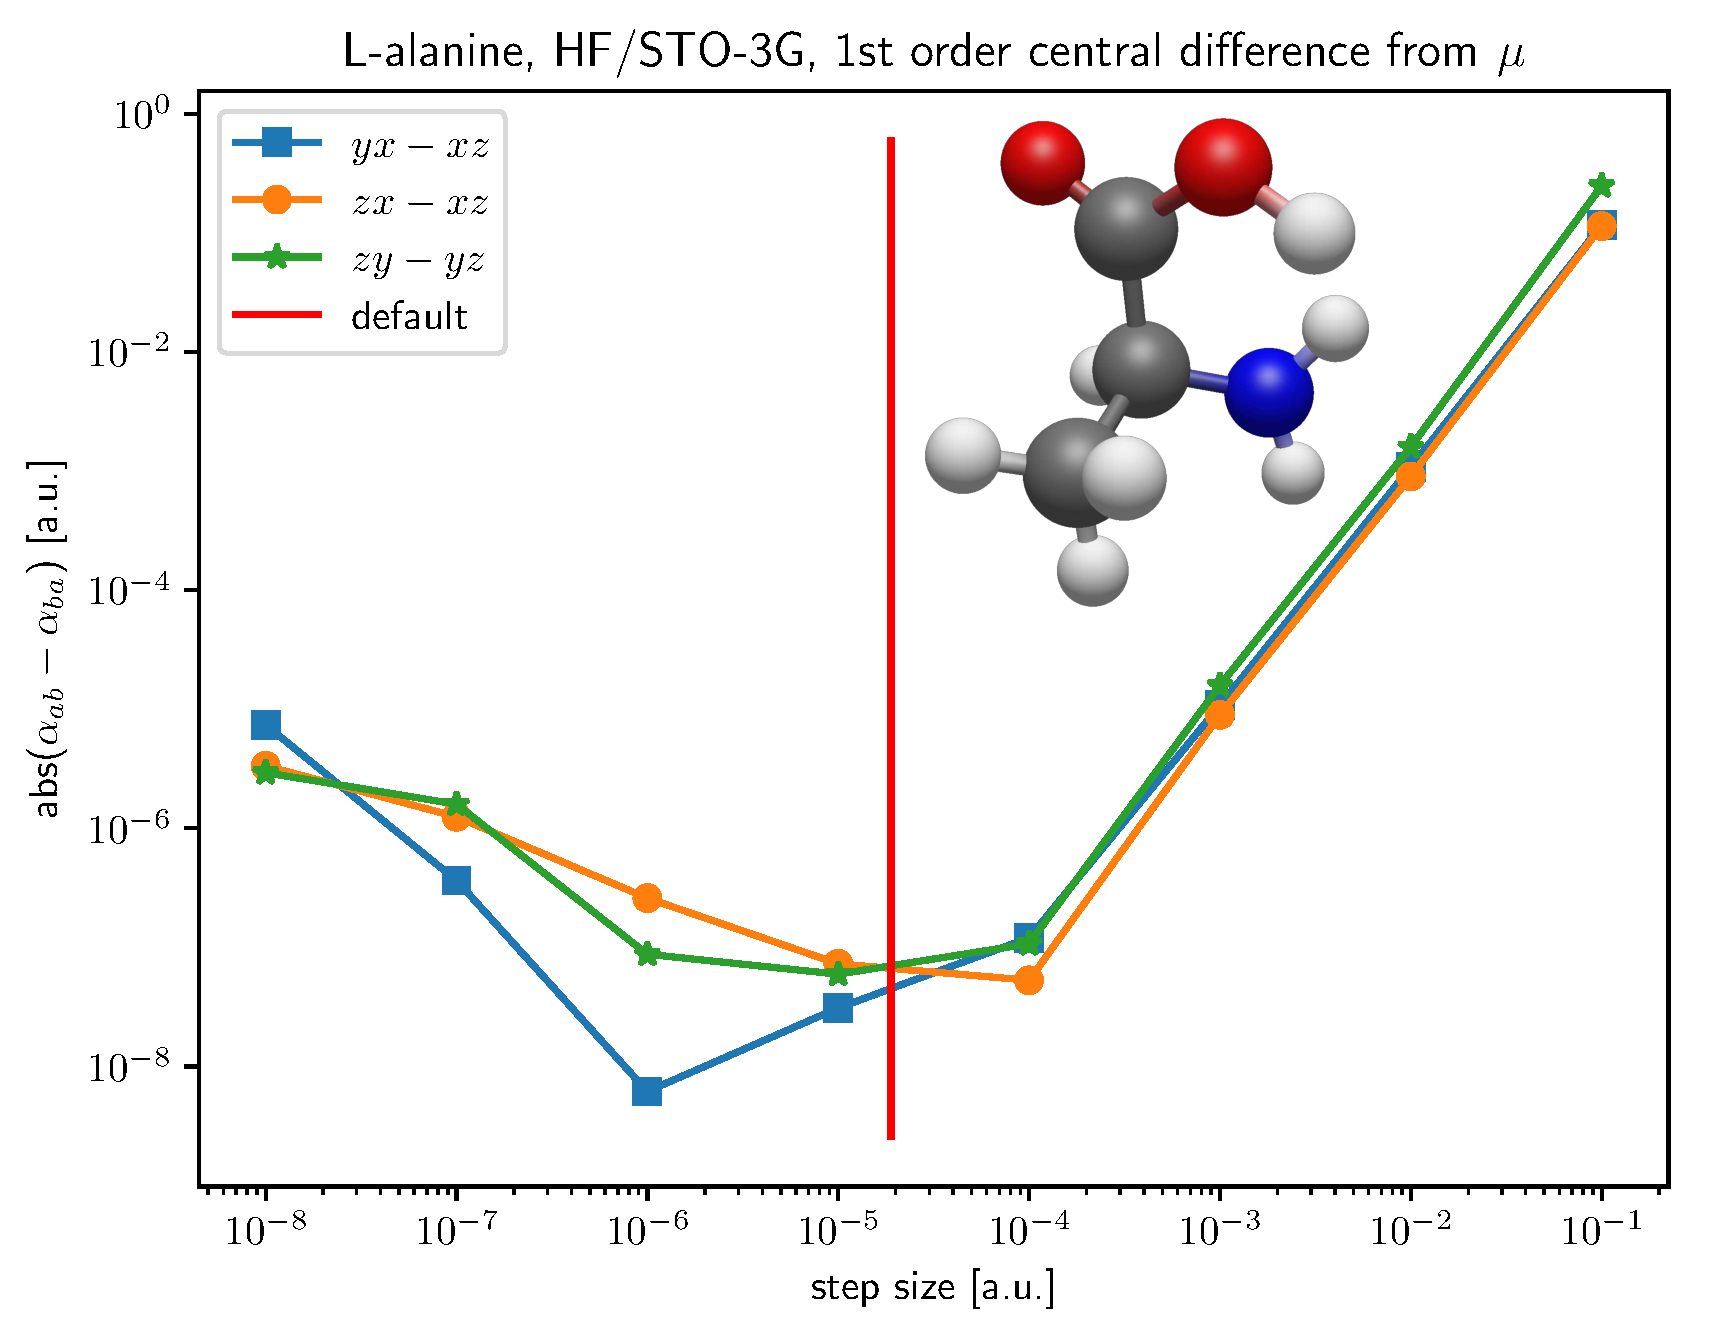
\includegraphics[width=\linewidth,keepaspectratio]{../diff_overlay2.pdf}
  \end{nscenter}
\end{frame}

\begin{frame}
  \frametitle{Spectroscopic properties are directly connected to energy derivatives}
  \begin{nscenter}
    \scriptsize
    \begin{tabulary}{1.00\linewidth}{rL}
      \toprule
      \textbf{Derivative} & \textbf{Molecular property} \\
      \midrule
      \(\frac{dE}{dF_{i}}\)                          & dipole moment; similarly,  multipole moments, electric field gradients, etc. \\
      \(\frac{dE}{dB_{\alpha}}\)                     & magnetic dipole moment and higher-order magnetic multipoles \\
      \(\frac{dE}{dX_{i}}\)                          & forces on nuclei; stationary points on potential energy surfaces, equilibrium and transition state structures \\
      \(\frac{dE}{dm_{K_{j}}}\)                      & spin density; hyperfine interaction constants \\
      \textcolor{AlertColor}{\(\frac{d^{2}E}{dF_{\alpha}dF_{\beta}}\)}       & \textcolor{AlertColor}{polarizability} \\
      \textcolor{AlertColor}{\(\frac{d^{2}E}{dX_{i}dX_{j}}\)}                & \textcolor{AlertColor}{harmonic force constants and vibrational frequencies} \\
      \(\frac{d^{2}E}{dX_{i}dF_{\alpha}}\)           & dipole derivatives; harmonic infrared intensities \\
      \(\frac{d^{2}E}{dB_{\alpha}dB_{\beta}}\)       & magnetizability \\
      \(\frac{d^{2}E}{dm_{K_{j}}dB_{\alpha}}\)       & nuclear magnetic shielding tensor; relative NMR shifts \\
      \(\frac{d^{2}E}{dI_{K_{i}}dI_{L_{j}}}\)        & indirect spin-spin coupling constant \\
      \(\frac{d^{2}E}{dB_{\alpha}dJ_{\beta}}\)       & rotational \textit{g}-tensor; rotational spectra in magnetic field \\
      \(\frac{d^{2}E}{dI_{K_{i}}dB_{\alpha}}\)       & nuclear spin-rotation tensor; fine structure in rotational spectra \\
      \(\frac{d^{2}E}{dS_{i}dB_{\alpha}}\)           & electronic \textit{g}-tensor \\
      % \(\frac{d^{3}E}{dX_{i}dF_{\alpha}dF_{\beta}}\) & polarizability derivative; Raman intensities \\
      % \(\frac{d^{3}E}{dF_{\alpha}d^{2}F_{\beta}}\)   & (first) electric hyperpolarizability \\
      % \(\frac{d^{3}E}{dX_{i}dX_{j}dX_{k}}\)          & cubic force constants; vibrational corrections to distances and rotational constants \\
      % \(\frac{d^{4}E}{dF_{\alpha}dF_{\beta}dF_{\gamma}dF_{\delta}}\) & (second) electric hyperpolarizability \\
      % \(\frac{d^{4}E}{dB_{\alpha}dB_{\beta}dB_{\gamma}dB_{\delta}}\) & (second) hypermagnetizability \\
      % \(\frac{d^{4}E}{dX_{i}dX_{j}dX_{k}dX_{l}}\)                    & quartic force constants; anharmonic corrections to vibrational frequencies \\
      % \(\frac{d^{4}E}{dF_{\alpha}dF_{\beta}dF_{\gamma}dX_{i}}\)      & hyper-Raman effects \\
      % \(\frac{d^{4}E}{dF_{\alpha}dF_{\beta}dX_{i}dX_{j}}\)           & Raman intensities for overtone and combination bands \\
      % \(\frac{d^{4}E}{dF_{\alpha}dF_{\beta}dB_{\gamma}dB_{\delta}}\) & Cotton\textendash{}Mutton effect \\
      ... & ... \\
      \bottomrule
    \end{tabulary}
  \end{nscenter}
\end{frame}

\section{Decomposition of general linear response properties}

\begin{frame}
  \frametitle{Solution: start from the framework of response theory}
  \note[item]{Many important molecular properties are calculated within the framework of linear response}
  Spectroscopic properties are directly connected to (linear) response functions:
  \note[item]{Linear response is named as such not due to the linear form of the equations, but because the perturbation is linear in strength. This strength may be constant, static, or time-independent, or it may be oscillating, dynamic, frequency-, or time-dependent.}
  \begin{table}
    \centering
    \begin{tabular}{ll}
      \toprule
      \textbf{Molecular property}       & \textbf{Linear response function} \\
      \midrule
      polarizability                    & \( \braket{\braket{\hat{\mu};\hat{\mu}}}_{\omega} \) \\
      magnetizability                   & \( \braket{\braket{\hat{m};\hat{m}}}_{0} \) \\
      optical rotation                  & \( \braket{\braket{\hat{\mu};\hat{m}}}_{\omega} \) \\
      electronic circular dichroism     & \( \braket{\braket{\hat{\mu};\hat{m}}}_{\omega_{f}} \) \\
      IR intensities                    & \( \braket{\braket{\hat{\mu};\partial\hat{H}_{0}/\partial R}}_{\omega} \) \\
      NMR spin-spin coupling constants  & \( \braket{\braket{\hat{h}_{\text{SD}};\hat{h}_{\text{SD}}}}_{0} \), \\
                                        & \( \braket{\braket{\hat{h}_{\text{FC}};\hat{h}_{\text{FC}}}}_{0} \), \\
                                        & \( \braket{\braket{\hat{h}_{\text{PSO}};\hat{h}_{\text{PSO}}}}_{0} \) \\
      NMR chemical shifts               & \( \braket{\braket{\hat{l}_{O};\hat{h}_{\text{PSO}}}}_{0} \) \\
      EPR \textit{g}-tensor             & \( \braket{\braket{\hat{l}_{O};\hat{h}_{\text{SOC}}}}_{0} \) \\
      ... & ... \\
      \bottomrule
    \end{tabular}
  \end{table}
\end{frame}

\begin{frame}
  \frametitle{The language of energy decomposition analysis can be applied to general response properties}
  We have already successfully translated
  \begin{equation*}
    \Delta E_{\text{int}} = \Delta E_{\text{geom}} + \Delta E_{\text{frz}} + \Delta E_{\text{pol}} + \Delta E_{\text{CT}}
  \end{equation*}
  into
  \begin{equation*}
    \omega_{\text{tot}} = \omega_{\text{free}} + \Delta \omega_{\text{geom}} + \Delta \omega_{\text{frz}} + \Delta \omega_{\text{pol}} + \Delta \omega_{\text{CT}}
  \end{equation*}
  Now do the same for linear response:
  \begin{equation*}
    \begin{aligned}
      \braket{\braket{\hat{P};\hat{Q}^{\omega}}}_{\text{tot}} = &\braket{\braket{\hat{P};\hat{Q}^{\omega}}}_{\text{free}} + \Delta \braket{\braket{\hat{P};\hat{Q}^{\omega}}}_{\text{geom}} \\
      &+ \Delta \braket{\braket{\hat{P};\hat{Q}^{\omega}}}_{\text{frz}} + \Delta \braket{\braket{\hat{P};\hat{Q}^{\omega}}}_{\text{pol}} + \Delta \braket{\braket{\hat{P};\hat{Q}^{\omega}}}_{\text{CT}}
    \end{aligned}
  \end{equation*}
\end{frame}

\begin{frame}
  \frametitle{Linear response in a nutshell}
  \note[item]{Walk us through the equations}
  The response of the property \(\hat{P}\) to the perturbation \(\hat{Q}\); for exact (orthogonal) states:
  \begin{equation*}
    \braket{\braket{\hat{P};\hat{Q}}}_{\omega_{Q}} = - \sum_{n>0} \left[ \frac{\braket{\Psi_{0}|\hat{P}|\Psi_{n}}\braket{\Psi_{n}|\hat{Q}|\Psi_{0}}}{E_{n} - E_{0} - \omega_{Q}} + \frac{\braket{\Psi_{0}|\hat{Q}|\Psi_{n}}\braket{\Psi_{n}|\hat{P}|\Psi_{0}}}{E_{n} - E_{0} + \omega_{Q}} \right]
  \end{equation*}
  In computable form,
  \begin{equation*}
    \braket{\braket{\hat{P}_{\alpha};\hat{Q}_{\beta}}}_{\omega_{Q}} = - \vect{P}_{\alpha}^{\dagger} \vect{G}^{-1} \vect{Q}_{\beta}
  \end{equation*}
  where
  \begin{equation*}
    (\vect{P}_{\alpha})_{ia} = -2 \braket{ i | \hat{P}_{\alpha} | a }
  \end{equation*}
  is a vector of property integrals in the occupied-virtual MO basis and \(\vect{G}^{-1}\) is the inverted \emph{orbital} Hessian. The key step is forming the response vector
  \begin{equation*}
    X_{ia} = G_{ia,jb}^{-1} Q_{jb}
  \end{equation*}
  \(X_{ia}\) is part of the orbital rotation matrix \(U_{ia}\) from coupled perturbed SCF (CPHF, CPKS).
\end{frame}

\begin{frame}
  \frametitle{Approach: take idea behind SCF(MI) and apply it to linear response \textrightarrow{} \textcolor{AlertColor}{LR(MI)}}
  Remove charge transfer: restrict excitations to only MOs within a fragment
  \note[item]{Did you attempt to reanalyze CO2 with this new method? [we discussed]}
  \begin{table}
    \centering
    \begin{tabular}{ll}
      Static response: & \(\braket{\braket{\hat{P};\hat{Q}}}_{0} = -(\vect{P})_{\textcolor{red}{ia}}(\vect{Q})_{\textcolor{red}{ia}}\) \\
      Response vector update: & \((\vect{X})_{ia} = (\vect{E}^{-1})_{ia,\textcolor{red}{jb}} \left[ (\vect{Q})_{\textcolor{red}{jb}} - (\vect{R})_{\textcolor{red}{jb}} \right]\)
    \end{tabular}
  \end{table}
  Work with the blocked response vector in a similar fashion to the Hamiltonian:
  \begin{table}
    \centering
    \begin{tabular}{ccc}
      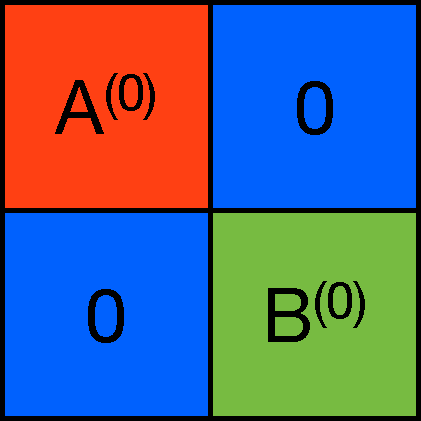
\includegraphics[scale=0.30]{./figures/block_1.pdf} & 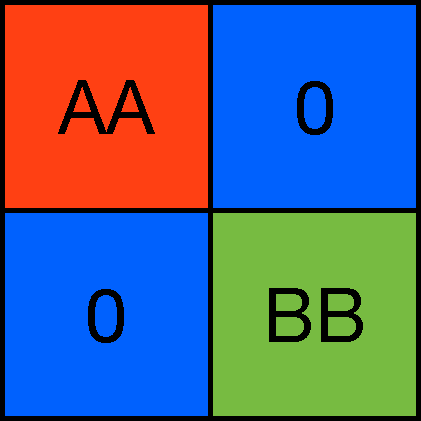
\includegraphics[scale=0.30]{./figures/block_2.pdf} & 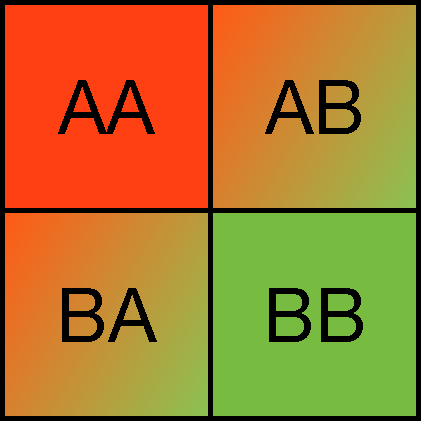
\includegraphics[scale=0.30]{./figures/block_3.pdf} \\
      frozen interaction & polarization & charge transfer \\
      \((\vect{1} - \vect{\sigma})^{\dagger} \vect{H}^{(0)} (\vect{1} - \vect{\sigma})\) & \((\vect{1} - \vect{\sigma})^{\dagger} \vect{H} (\vect{1} - \vect{\sigma})\) & \(\vect{H}\) \\
      \((\vect{1} - \vect{\sigma})^{\dagger} \vect{X}^{(0)} (\vect{1} - \vect{\sigma})\) & \((\vect{1} - \vect{\sigma})^{\dagger} \vect{X} (\vect{1} - \vect{\sigma})\) & \(\vect{X}\)
    \end{tabular}
  \end{table}
\end{frame}

\begin{frame}
  \frametitle{LR(MI) identifies which fragments are important for charge transfer}
  \begin{table}
    \centering
    \begin{tabular}{ccc}
      \includegraphics[scale=0.30]{./figures/block_1.pdf} & \includegraphics[scale=0.30]{./figures/block_2.pdf} & \includegraphics[scale=0.30]{./figures/block_3.pdf} \\
      frozen interaction & polarization & charge transfer \\
      \((\vect{1} - \vect{\sigma})^{\dagger} \vect{H}^{(0)} (\vect{1} - \vect{\sigma})\) & \((\vect{1} - \vect{\sigma})^{\dagger} \vect{H} (\vect{1} - \vect{\sigma})\) & \(\vect{H}\) \\
      \((\vect{1} - \vect{\sigma})^{\dagger} \vect{X}^{(0)} (\vect{1} - \vect{\sigma})\) & \((\vect{1} - \vect{\sigma})^{\dagger} \vect{X} (\vect{1} - \vect{\sigma})\) & \(\vect{X}\)
    \end{tabular}
  \end{table}
  Selectively allow charge transfer from a single fragment to all others:
  \begin{table}
    \centering
    \begin{tabular}{cc}
      \includegraphics[scale=0.30]{./figures/block_ab_0.pdf} & \includegraphics[scale=0.30]{./figures/block_ba_0.pdf} \\
      frz + pol + CT(A \(\rightarrow\) all) & frz + pol + CT(B\(\rightarrow\) all)
    \end{tabular}
  \end{table}
\end{frame}

\begin{frame}
  \frametitle{Numerical benchmarks using static electric dipole polarizabilities}
  \note[item]{Why polarizability? can compare to finite difference numerical derivatives}
  \note[item]{Why static? static helps provide the connection between analytic derivatives and response theory}
  As an energy derivative,
  \begin{equation*}
    \alpha_{rs} = - \left. \frac{\text{d}^{2}E}{\text{d}F_{r}\text{d}F_{s}} \right|_{\mathbf{F}=\mathbf{0}}
  \end{equation*}
  which is equivalent to the response theory formulation
  \begin{equation*}
    \alpha_{rs} = - \braket{\braket{\hat{\mu}_{r};\hat{\mu}_{s}}}_{0}
  \end{equation*}
  The test system is the argon\textemdash{}lithium cation dimer, \arlidimer{}.
  \begin{figure}
    \centering
    \includegraphics[scale=0.15]{./figures/Qchem-logo.png}
  \end{figure}
  \nmfootfullcite{Berquist2018}
\end{frame}

\begin{frame}
  \frametitle{LR(MI) analytic static polarizabilities are quantitatively correct compared to finite difference}
  \note[item]{This shows the correctness of our implementation}
  \note[item]{Confirm correctness before scientific result}
  \note[item]{deviation between implementations occurs in the electron density penetration region, where ALMO is not expected to be valid anyway}
  \begin{nscenter}
    \includegraphics[scale=0.65]{./figures/almo_analytic_vs_numerical_onaxis_projected_short_def2-SVPD.pdf}
  \end{nscenter}
  {\tiny HF/def2-SVPD}
\end{frame}

\begin{frame}
  \frametitle{LR(MI) polarizabilities have physically-correct long-range asymptotic behavior}
  \begin{nscenter}
    \includegraphics[scale=0.65]{./figures/long_convergence_behavior_onaxis_def2-SVPD.pdf}
  \end{nscenter}
  {\tiny HF/def2-SVPD}
\end{frame}

\begin{frame}
  \frametitle{LR(MI) allows for decomposing response properties analogously to ALMO-EDA}
  \begin{nscenter}
    \includegraphics[scale=0.70]{./figures/bar_combined.pdf}
  \end{nscenter}
\end{frame}

\begin{frame}
  \frametitle{LR(MI) confirms charge transfer is more significant from argon than lithium}
  \begin{nscenter}
    \includegraphics[scale=0.70]{./figures/bar_virtual_combined.pdf}
  \end{nscenter}
\end{frame}

\begin{frame}
  \frametitle{LR(MI) reveals charge transfer is important for both response and the underlying wavefunction}
  \begin{nscenter}
    \includegraphics[scale=0.70]{./figures/bar_mechanisms_combined.pdf}
  \end{nscenter}
\end{frame}

\begin{frame}
  \frametitle{LR(MI) is in libresponse, an open-source library}
  \note[item]{working on Psi4 plugin}
  \note[item]{"Is available online" -- **you** put these online, right? The way you described it makes it sound like someone else already had them up. Use the active voice (even if it's 1st person plural "we placed these online ...")}
  \scriptsize
  \begin{nscenter}
    \includegraphics[scale=0.30]{./figures/libresponse_top.pdf} \\
    \includegraphics[scale=0.32]{./figures/libresponse_bottom.pdf} \\
    BSD 3-clause license \\
    \url{https://github.com/LambrechtLab/libresponse} \\
    \url{https://github.com/berquist/pyresponse}
  \end{nscenter}
\end{frame}

\section{Reference and tutorial implementations of quantum chemical methods}

\begin{frame}
  \frametitle{\pfn{} provides a modern ecosystem for quantum chemical method development}
  \begin{nscenter}
    \includegraphics[width=\linewidth,keepaspectratio]{./figures/psi4numpy_ecosystem22.pdf}
  \end{nscenter}
\end{frame}

\begin{frame}
  \frametitle{\pfn{} is an ideal platform for teaching about \textit{ab initio} spectroscopy}
  \begin{nscenter}
    \includegraphics[width=\linewidth,keepaspectratio]{./figures/psi4numpy_notebook_1.png}
  \end{nscenter}
\end{frame}

\begin{frame}
  \frametitle{Jupyter Notebooks allow mixing of concepts, equations, and code in an exploratory environment}
  \begin{nscenter}
    \includegraphics[width=\linewidth,keepaspectratio]{./figures/psi4numpy_notebook_2.png}
  \end{nscenter}
\end{frame}

\begin{frame}
  \frametitle{\pfn{} is welcoming to external contributors}
  \begin{nscenter} % < 0.20
    \includegraphics[width=\linewidth,keepaspectratio]{./figures/psi4numpy_github.png}
    {\scriptsize \url{https://github.com/psi4/psi4numpy/}}
  \end{nscenter}
  \nmfootfullcite{Smith2018}
\end{frame}

\begin{frame}
  \frametitle{Future extensions}
  \begin{itemize}
  \item Geometric perturbations: applications for piezoelectric materials
  \item Frozen interaction in \libresponse{}
  \item Incorporate dispersion via 2nd-generation ALMO-EDA
  \item Non-linear response: \(\beta(-(\omega_{1}+\omega_{2});\omega_{1},\omega_{2})\) is from quadratic response, \(\gamma(-(\omega_{1}+\omega_{2}+\omega_{3});\omega_{1},\omega_{2},\omega_{3})\) is from cubic response, \dots
  \item ALMO/SCF(MI) in \pfn{}
  \item Second-order polarization propagator approximation (SOPPA) in \pfn{}
  \item \dots
  \end{itemize}
\end{frame}

\begin{frame}
  \frametitle{Conclusions}
  Thesis: It is possible to identify the contribution of specific molecular interactions to spectroscopic response.
  \begin{itemize}
  \item Decomposition of molecular properties is part of a larger workflow for building structure-spectra-property relationships
  \item Charge transfer is a primary contributor to the infrared signature of \ce{CO2} in ILs
  \item \libresponse{} is a general (linear) response library that allows decomposition of complex molecular \& materials functions into well-defined chemical contributions derived from first principles
  \item Open-source development is a valid path forward for quantum chemical method development
  \end{itemize}
\end{frame}

\begin{frame}
  \frametitle{Acknowledgments}
  \begin{columns}
    \column{0.65\textwidth}
    \begin{minipage}{1.0\linewidth}
      \scriptsize
      \begin{itemize}
      \item Prof. Daniel Lambrecht
      \item Prof. Sean Garrett-Roe
      \item Prof. Ken Jordan
      \item Prof. David Yaron (CMU)
      \item Evgeny Epifanovsky (Q-Chem)
      \item Thomas Brinzer (Pitt)
      \item Daniel Smith (MolSSI, Psi4)
      \item Clyde Daly (Notre Dame)
      \item Prof. Steve Corcelli (Notre Dame)
      \end{itemize}
      \includegraphics[scale=0.38]{./figures/lambrecht_group.png}
    \end{minipage}
    \column{0.35\textwidth}
    \begin{minipage}{1.0\linewidth}
      \centering
      \includegraphics[width=1.00\linewidth,keepaspectratio]{./figures/Qchem-logo.png}
      \includegraphics[width=0.90\linewidth,keepaspectratio]{./figures/PQI-Letter-Logo-black.png}
      \includegraphics[width=0.85\linewidth,keepaspectratio]{./figures/logo_crc.jpg}
      \includegraphics[width=0.95\linewidth,keepaspectratio]{./figures/logo_novartis.png}
      \includegraphics[scale=0.15]{./figures/logo_cclib.png}
      \includegraphics[width=1.00\linewidth,keepaspectratio]{./figures/psi4numpybanner_eqn.png}
      \includegraphics[width=0.95\linewidth,keepaspectratio]{./figures/logo_molssi_text.jpg}
    \end{minipage}
  \end{columns}
\end{frame}

\begin{frame}
  \frametitle{Thank you}
  \scriptsize
  \begin{enumerate}
  \item \fullcite{Berquist2014}
  \item \fullcite{Shao2015}
  % \item {\setbeamercolor{bibliography entry author}{fg=Green}\fullcite{Brinzer2015}}
  \item \fullcite{Brinzer2015}
  \item \fullcite{Daly2016}
  \item \fullcite{Berquist2017}
  \item \fullcite{Brinzer2017}
  \item \fullcite{Smith2018}
  % \item {\setbeamercolor{bibliography entry author}{fg=Green}\fullcite{Berquist2018}}
  \item \fullcite{Berquist2018}
  \item \fullcite{Jakubek2018}
  \end{enumerate}
\end{frame}

\appendix

\begin{frame}
  \frametitle{The calculated solvatochromic shift ordering may result from a minimal treatment of the environment}
  \begin{nscenter}
    \includegraphics[width=\linewidth,keepaspectratio]{./figures/updated_methods.pdf}
  \end{nscenter}
\end{frame}

\begin{frame}
  \frametitle{Complementary occupied-virtual pairs (COVPs) are a compact representation of donor/acceptor orbitals}
  \begin{figure}
    \centering
    \begin{subfigure}[b]{0.50\linewidth}
      \includegraphics[width=\linewidth,keepaspectratio,natwidth=601,natheight=535]{./figures/PF6.to_CO2.1.png}
      \caption*{From \ce{[PF6]-} to \ce{CO2}}
    \end{subfigure}%
    \begin{subfigure}[b]{0.50\linewidth}
      \includegraphics[width=\linewidth,keepaspectratio,natwidth=586,natheight=538]{./figures/PF6.from_CO2.1.png}
      \caption*{From \ce{CO2} to \ce{[C1C1im]+}}
    \end{subfigure}
  \end{figure}
  \begin{nscenter}
    \(\Delta E_{\text{CT}} = \mathrm{Tr}[\mathbf{X}_{ov}\mathbf{F}_{vo}^{\text{ALMO}}] + \Delta E_{\text{HO}}\)
  \end{nscenter}
  \nmfootfullcite{Ramos-Cordoba2011}
\end{frame}

\begin{frame}
  \frametitle{Implementation: working equations (RHF)}
  \begin{align*}
    \Delta_{ia} &= \epsilon_{a} - \epsilon_{i} \\
    A_{ia,jb}^{s} &= \Delta_{ia}\delta_{ia,jb} + 2(ia|jb) - (ij|ab) \\
    B_{ia,jb}^{s} &= 2(ia|jb) - (ib|ja) \\
    A_{ia,jb}^{t} &= \Delta_{ia}\delta_{ia,jb} - (ij|ab) \\
    B_{ia,jb}^{t} &= - (ib|ja) \\
    ^{\text{RR}}\vect{G}^{uu} &= (\vect{A}^{u} + \vect{B}^{u}) \\
    ^{\text{II}}\vect{G}^{uu} &= (\vect{A}^{u} - \vect{B}^{u})
  \end{align*}
  \scriptsize
  \begin{itemize}
  \item \(\vect{G}\) gives orbital rotation Hessians, equivalen to the random phase approximation (RPA) equations \\
  \item R, I: real, imaginary perturbations \(\rightarrow\) electric and magnetic Hessians \\
  \item setting \(\vect{B} = \vect{0}\) gives the Tamm-Dancoff approximation (TDA) \\
  \item setting \( G_{ia,jb} = \Delta_{ia}\delta_{ia,jb} \) gives uncoupled Hartree-Fock \\
  \item \(s,t\): singlet (spin-conserving) and triplet (altering) operators \\
  \item \(i,j\): occupied MOs, \(a,b\): virtual MOs
  \end{itemize}
\end{frame}

\begin{frame}
  \frametitle{libresponse implementation: AO-direct algorithm}
  Rather than explicitly forming \(G_{ia,jb}\), inverting it, and contracting with \(Q_{jb}\) to form the response vector \(X_{ia}\), the solution is found iteratively (example is RPA/singlet):
  \begin{equation*}
    X_{ia}^{(\zeta+1)} \leftarrow \frac{Q_{jb} - \left[4(ia|jb) - (ij|ab) - (ib|ja)\right] X_{jb}^{(\zeta)}}{\Delta_{ia}}
  \end{equation*}
  The uncoupled result comes from the initial guess, when \(X_{ia}^{(0)} = 0\):
  \begin{equation*}
    X_{ia}^{(1)} = \frac{Q_{ia}}{\Delta_{ia}}
  \end{equation*}
  Convergence is usually accelerated with CG, DIIS, ...
\end{frame}

\begin{frame}
  \frametitle{libresponse implementation: AO-direct algorithm}
  \scriptsize
  The key step in each iteration is forming the matrix-vector product
  \begin{equation*}
    (\vect{A}+\vect{B})_{ia,jb}X_{jb} = \left[4(ia|jb) - (ij|ab) - (ib|ja)\right] X_{jb}^{(\zeta)}
  \end{equation*}
  which is found through back-transforming to the AO basis, starting from the generalized density:
  \begin{equation*}
    D_{\lambda\sigma}^{X} \equiv C_{\lambda j} X_{jb} C_{\sigma b}
  \end{equation*}
  which is contracted with two-electron integrals formed either exactly or through approximate methods (RI, ...):
  \begin{align*}
    (\vect{A}+\vect{B})_{ia,jb}X_{jb} &= C_{\mu i} \left\{ 4(\mu\nu|\lambda\sigma)D_{\lambda\sigma}^{X} - (\mu\lambda|\nu\sigma)D_{\lambda\sigma}^{X} - (\mu\sigma|\lambda\nu)D_{\lambda\sigma}^{X} \right\} C_{\nu a} \\
    &= C_{\mu i} \left\{ 4J_{\mu\nu}^{X} - K_{\mu\nu}^{X} - K_{\nu\mu}^{X} \right\} C_{\nu a}
  \end{align*}
  In \texttt{libint}, this is \texttt{JobNum = 30}.
\end{frame}

\begin{frame}[fragile]
  \frametitle{libresponse/Q-Chem implementation: library usage}
  \texttt{responseman} is a thin wrapper around \texttt{libresponse}, and is not meant to calculate final properties (similar to \texttt{**RESPONSE} vs. \texttt{**PROPERTIES} in DALTON). \\
  \begin{minted}[autogobble]{c++}
void solve_linear_response(
    arma::cube &results,
    MatVec_i *matvec,
    SolverIterator_nonorthogonal *solver_iterator,
    const arma::cube &C,
    const arma::umat &fragment_occupations,
    const arma::uvec &occupations,
    const arma::cube &F,
    const arma::mat &S,
    const std::vector<double> &omega,
    std::vector<operator_spec> &operators,
    const configurable &cfg
    );
  \end{minted}
\end{frame}

\begin{frame}[fragile]
  \frametitle{libresponse/Q-Chem implementation: integral engine}
  \scriptsize
  \begin{minted}[linenos,gobble=0,mathescape]{c++}
if (ints_engine == "libfock" || ints_engine == "both") {
    matvec_libfock = new MatVec_libfock();
    libqints::basis_1e1c_cgto<double> b1;
    libqints::qchem::bagen_1e1c_cgto_qchem(b1);
    matvec_libfock->init(b1, mem_mb);
    matvec = matvec_libfock;
} else if (ints_engine == "qchem" || ints_engine == "both") {
    matvec_qchem = new MatVec_qchem();
    matvec_qchem->init();
    matvec = matvec_qchem;
} else
    ...
  \end{minted}
\end{frame}

\begin{frame}
  \frametitle{libresponse/Q-Chem current capabilities}
  QC methods:
  \begin{itemize}
  \item RHF, UHF references \(\rightarrow\) DALTON is ROHF, is this the first true general UHF linear response code?
  \item All SCF-based methods excluding perturbative corrections (no double-hybrid DFT)
  \end{itemize}
  Operators (\texttt{libint}):
  \begin{itemize}
  \item dipole (length), quadrupole at arbitrary origin
  \item Fermi contact at nuclear positions
  \item dipole velocity/linear momentum
  \item angular momentum at arbitrary origin
  \item one-electron spin-orbit over all nuclei w/ arbitrary charges
  \item arbitrary-order electric field multipoles at arbitrary origin
  \item spin dipole at nuclear positions
  \end{itemize}
  Properties via \texttt{responseman}:
  \begin{itemize}
  \item static polarizability
  \end{itemize}
\end{frame}

\begin{frame}
  \frametitle{libresponse/Q-Chem planned capabilities}
  \begin{itemize}
  \item Convergence acceleration beyond DIIS
  \item Density functionals with nonlocal dispersion
  \item Operators: two-electron spin-orbit
  \item time-dependent/dynamic properties
  \item residues \(\rightarrow\) transition moments
    \begin{equation*}
      \lim_{\omega_{1} \to \omega_{n0}} (\omega_{n0} - \omega_{1}) \braket{\braket{\hat{P};\hat{Q}^{\omega_{1}}}} = \braket{0|\hat{P}|n} \braket{n|\hat{Q}^{\omega_{1}}|0}
    \end{equation*}
  \item complex response via \texttt{gen\_scfman}
    \begin{equation*}
    \braket{\braket{\hat{P};\hat{Q}}}_{\omega_{Q}} = \sum_{n>0} \left[ \frac{\braket{0|\hat{P}|n}\braket{n|\hat{Q}|0}}{\omega_{n0} - \omega_{Q} - i\gamma_{n0}} + \frac{\braket{0|\hat{Q}|n}\braket{n|\hat{P}|0}}{\omega_{n0} + \omega_{Q} + i\gamma_{n0}} \right]
    \end{equation*}
  \item quadratic response \(\braket{\braket{\hat{P};\hat{Q},\hat{R}}}_{\omega_{Q},\omega_{R}}\)
  \end{itemize}
\end{frame}

\begin{frame}[fragile]
  \begin{minted}[gobble=4]{python}
    def solve_dynamic_iterative(self, omega=0.0, maxiter=20, conv=1.e-9, use_diis=True):

        # Init JK object
        jk = psi4.core.JK.build(self.scf_wfn.basisset())
        jk.initialize()

        # Add blank matrices to the JK object and NumPy hooks to
        # C_right; there are 6 sets of matrices to account for X and Y
        # vectors separately.
        npC_right = []
        for xyz in range(6):
            jk.C_left_add(self.Co)
            mC = psi4.core.Matrix(self.nbf, self.nocc)
            npC_right.append(np.asarray(mC))
            jk.C_right_add(mC)
  \end{minted}
\end{frame}

\begin{frame}[fragile]
  \frametitle{Psi4NumPy reference implementation is ``pseudocode'' that exactly mirrors the response equations}
  \begin{minted}[gobble=4]{python}
        # Build initial guess, previous vectors, diis object, and C_left updates
        x_l, x_r = [], []
        x_l_old, x_r_old = [], []
        diis_l, diis_r = [], []
        ia_denom_l = self.epsilon[self.nocc:] - self.epsilon[:self.nocc].reshape(-1, 1) - omega
        ia_denom_r = self.epsilon[self.nocc:] - self.epsilon[:self.nocc].reshape(-1, 1) + omega
        for xyz in range(3):
            x_l.append(self.dipoles_xyz[xyz] / ia_denom_l)
            x_r.append(self.dipoles_xyz[xyz] / ia_denom_r)
            x_l_old.append(np.zeros(ia_denom_l.shape))
            x_r_old.append(np.zeros(ia_denom_r.shape))
  \end{minted}
  \begin{align*}
    X_{ia}^{\text{left};(0)} &= Q_{ia} / (E_{a} - E_{i} - \omega) \\
    X_{ia}^{\text{right};(0)} &= Q_{ia} / (E_{a} - E_{i} + \omega)
  \end{align*}
\end{frame}

\begin{frame}[fragile]
  \frametitle{Psi4NumPy: iterative static linear response}
  \begin{minted}[gobble=4]{python}
        for CPHF_ITER in range(1, maxiter + 1):

            # Update jk's C_right
            for xyz in range(3):
                npC_right[xyz][:] = Cv.dot(self.x[xyz].T)

            # Compute JK objects
            jk.compute()

            # Update amplitudes
            for xyz in range(3):
                # Build J and K objects
                J = np.asarray(jk.J()[xyz])
                K = np.asarray(jk.K()[xyz])

                # Bulid new guess
                X = self.dipoles_xyz[xyz].copy()
                X -= (Co.T).dot(4 * J - K.T - K).dot(Cv)
                X /= ia_denom
  \end{minted}
  \begin{equation*}
    X_{ia}^{(\zeta+1)} \leftarrow \frac{Q_{jb} - \left[4(ia|jb) - (ij|ab) - (ib|ja)\right] X_{jb}^{(\zeta)}}{\Delta_{ia}}
  \end{equation*}
\end{frame}

\begin{frame}[fragile]
  \frametitle{Psi4NumPy: iterative dynamic linear response}
  \begin{minted}[gobble=4]{python}
        for CPHF_ITER in range(1, maxiter + 1):
            # Update jk's C_right; ordering is Xx, Xy, Xz, Yx, Yy, Yz
            for xyz in range(3):
                npC_right[xyz][:] = Cv.dot(x_l[xyz].T)
                npC_right[xyz + 3][:] = Cv.dot(x_r[xyz].T)

            # Perform generalized J/K build
            jk.compute()

            # Update amplitudes
            for xyz in range(3):
                # Build J and K objects
                J_l = np.asarray(jk.J()[xyz]); J_r = np.asarray(jk.J()[xyz + 3])
                K_l = np.asarray(jk.K()[xyz]); K_r = np.asarray(jk.K()[xyz + 3])

                # Bulid new guess
                X_l = self.dipoles_xyz[xyz].copy(); X_r = self.dipoles_xyz[xyz].copy()
                X_l -= (Co.T).dot(2 * J_l - K_l).dot(Cv)
                X_r -= (Co.T).dot(2 * J_r - K_r).dot(Cv)
                X_l /= ia_denom_l; X_r /= ia_denom_r
  \end{minted}
  \begin{equation*}
    X_{ia}^{(\zeta+1)} \leftarrow \frac{Q_{jb} - \left[4(ia|jb) - (ij|ab) - (ib|ja)\right] X_{jb}^{(\zeta)}}{\Delta_{ia}}
  \end{equation*}
\end{frame}

\begin{frame}
  \frametitle{LR(MI) analytic static polarizabilities are quantitatively correct compared to finite difference results at short range}
  \note[item]{This shows the correctness of our implementation}
  \note[item]{Confirm correctness before scientific result}
  \note[item]{deviation between implementations occurs in the electron density penetration region, where ALMO is not expected to be valid anyway}
  \begin{nscenter}
    \includegraphics[scale=0.65]{./figures/almo_analytic_vs_numerical_onaxis_projected_short_def2-SVP.pdf}
  \end{nscenter}
  {\tiny HF/def2-SVP}
\end{frame}

\begin{frame}
  \frametitle{LR(MI) polarizabilities have physically-correct long-range asymptotic behavior}
  \begin{nscenter}
    \includegraphics[scale=0.65]{./figures/long_convergence_behavior_onaxis_def2-SVP.pdf}
  \end{nscenter}
  {\tiny HF/def2-SVP}
\end{frame}

\begin{frame}
  \frametitle{LR(MI) is BSSE-free by construction: def2-SVP}
  \begin{nscenter}
    \includegraphics[scale=0.50]{./figures/almo_vs_bsse_canonical_onaxis_projected_short_def2-SVP.pdf}
  \end{nscenter}
  \scriptsize
  \begin{equation*}
    \alpha^{\text{BSSE-corrected}} = \alpha^{AB}(AB) - \left[ \left( \alpha^{A}(AB) - \alpha^{A}(A) \right) + \left( \alpha^{B}(AB) - \alpha^{B}(B) \right) \right]
  \end{equation*}
  HF/def2-SVP
\end{frame}

\begin{frame}
  \frametitle{LR(MI) is BSSE-free by construction: def2-SVPD}
  \begin{nscenter}
    \includegraphics[scale=0.50]{./figures/almo_vs_bsse_canonical_onaxis_projected_short_def2-SVPD.pdf}
  \end{nscenter}
  \scriptsize
  \begin{equation*}
    \alpha^{\text{BSSE-corrected}} = \alpha^{AB}(AB) - \left[ \left( \alpha^{A}(AB) - \alpha^{A}(A) \right) + \left( \alpha^{B}(AB) - \alpha^{B}(B) \right) \right]
  \end{equation*}
  HF/def2-SVPD
\end{frame}

\begin{frame}
  \frametitle{Polarizability at short distance, def2-SVP}
  \begin{figure}
    \centering
    \includegraphics[width=\linewidth,keepaspectratio]{../paper_04/polar_onaxis_projected_short_def2-SVP.pdf}
    \caption*{\arlidimer{}, HF/def2-SVP}
  \end{figure}
\end{frame}

\begin{frame}
  \frametitle{Polarizability at short distance, def2-SVPD}
  \begin{figure}
    \centering
    \includegraphics[width=\linewidth,keepaspectratio]{../paper_04/polar_onaxis_projected_short_def2-SVPD.pdf}
    \caption*{\arlidimer{}, HF/def2-SVPD}
  \end{figure}
\end{frame}

\begin{frame}
  \frametitle{Polarizability at long distance, def2-SVP}
  \begin{figure}
    \centering
    \includegraphics[width=\linewidth,keepaspectratio]{../paper_04/polar_onaxis_projected_long_def2-SVP.pdf}
    \caption*{\arlidimer{}, HF/def2-SVP}
  \end{figure}
\end{frame}

\begin{frame}
  \frametitle{Polarizability at long distance, def2-SVPD}
  \begin{figure}
    \centering
    \includegraphics[width=\linewidth,keepaspectratio]{../paper_04/polar_onaxis_projected_long_def2-SVPD.pdf}
    \caption*{\arlidimer{}, HF/def2-SVPD}
  \end{figure}
\end{frame}

\immediate\closeout\tempfile

\end{document}
